% !TeX program = xelatex
\documentclass[11pt]{article}
\usepackage[a4paper,margin=25mm]{geometry}
\usepackage{fontspec,libertine,amsmath,amssymb,amsthm,booktabs,array,longtable,graphicx}
\usepackage[hidelinks]{hyperref}
\setlength{\emergencystretch}{2em}
\hypersetup{pdftitle={FG-DUCS: Supplementary Proofs and Tables},pdfauthor={Anonymous Authors}}
\newcommand{\Post}{\mathsf{Post}}
\newcommand{\Safe}{\mathsf{Safe}}
\newcommand{\Goal}{Q_{\mathrm{goal}}}
\newcommand{\rank}{\mathsf{rk}}
\newcommand{\Reach}{\mathsf{Reach}}
\newcommand{\Init}{\mathsf{Init}}
\newcommand{\ActT}{\mathsf{ActiveM}}
\newcommand{\SuccSet}{\mathsf{Succ}}
\newcommand{\En}{\mathsf{En}}
\newcommand{\Ev}{\mathsf{Ev}}
\newcommand{\Cand}{\mathsf{Cand}}
\newcommand{\Sigmauc}{\Sigma_{\mathrm{uc}}}
\newcommand{\Sigmac}{\Sigma_{\mathrm{c}}}
\newcommand{\SigmaU}{\Sigma_{\mathrm{upd}}}
\newcommand{\ustart}[1]{\mathsf{start}(#1)}
\newcommand{\ustop}[1]{\mathsf{stop}(#1)}
\renewcommand{\thesection}{S\arabic{section}}
\renewcommand{\thetable}{S\arabic{table}}
\renewcommand{\thefigure}{S\arabic{figure}}
\newtheorem{lemma}{Lemma}[section]
\newtheorem{theorem}[lemma]{Theorem}
\newtheorem{proposition}[lemma]{Proposition}
\title{Fine-Grained Dynamic Update Controller Synthesis\\Supplementary Proofs and Tables}
\author{Anonymous Authors}
\date{}
% Derived from validated returned raw; elapsed/RSS are single-trial references, not medians.
\providecommand{\ADDirectFullWins}{14}
\providecommand{\ADDirectFullTimeouts}{13}
\providecommand{\ADWorkflowCapSeconds}{1200}
\providecommand{\ADWorkflowElapsedSeconds}{1201.7}
\providecommand{\ADWorkflowPeakRSSGiB}{13.9}
\providecommand{\ADPCCapSeconds}{3600}
\providecommand{\ADPCElapsedSeconds}{3605.2}
\providecommand{\ADPCPeakRSSGiB}{67.1}

% Generated from validated Xeon raw; do not edit.
\newcommand{\LFConditions}{21}
\newcommand{\LFFamilies}{8}
\newcommand{\LFPublishedWins}{21}
\newcommand{\LFForkWins}{16}
\newcommand{\LFSizeMatches}{15}
\newcommand{\LFSizeMismatches}{1}
\newcommand{\LFUnmeasured}{5}
\newcommand{\LFParserNM}{3}
\newcommand{\LFInstrumentationNM}{2}
\newcommand{\LFRailcabStateDelta}{5}
\newcommand{\LFRailcabTransitionDelta}{7}

\providecommand{\RSMonitorOccurrences}{273}
\providecommand{\RSClassifiedOccurrences}{273}
\providecommand{\RSFluentDeterminedOccurrences}{0}
\providecommand{\RSExactOccurrences}{0}
\providecommand{\RSUntestedOccurrences}{273}
\providecommand{\RSUnclassifiedOccurrences}{0}
\providecommand{\RSNewOccurrences}{138}
\providecommand{\RSUpdateOccurrences}{135}
\providecommand{\RSAExactOccurrences}{138}
\providecommand{\RSEExactOccurrences}{0}
\providecommand{\RSAEUnverifiedOccurrences}{135}
\providecommand{\RSEObserverSyncOccurrences}{89}
\providecommand{\RSEResetConsistentOccurrences}{135}
\providecommand{\RSEAHExactOccurrences}{89}
\providecommand{\RSAHEUnverifiedOccurrences}{46}
\providecommand{\RSAInclusionNew}{138}
\providecommand{\RSAExactNew}{138}
\providecommand{\RSEExactUpd}{89}
\providecommand{\RSUpdOccurrences}{135}
\providecommand{\RSAUnverifiedNew}{0}
\providecommand{\RSEUnverifiedUpd}{46}

\begin{document}
\maketitle
This supplement uses the finite contract, four successor rules, and algorithm in the main paper. Its proofs use the confirmed non-preemptive rule: update events have no successor whenever a physical uncontrollable event is enabled. Goals are safe, uncontrollable-quiescent states with all update events completed and a compatible supplied endpoint. No fairness assumption is added. Section~S4 reports completed correctness/capability and Xeon results, retaining unresolved outcomes and original trial provenance.

\section{Granularity and observation witnesses}
\label{supp:witnesses}
The main paper contains all primitive transitions, total-monitor conventions, controllers, initialization maps, roots, and load targets for $\mathcal W_{\rm cell}$, $\mathcal W_b$, and $\mathcal W_r$. Thus each witness can be reconstructed without this supplement. Here we give the complete arguments and clarify how the smaller executable fixtures relate to them.

\subsection{Embedding and Production Cell}
For a global-boundary input with a single component $\star$, identify its old/new component states with the corresponding old/new product states. Carry monitor states and pending requirement operations unchanged. The map on update states is a bijection. The ordinary rule synchronizes the same transitions, the transfer rule applies the same global relation, and requirement stop/start applies the same monitor update and initialization. The sets of physical uncontrollables coincide, so the non-preemption guard also coincides. Safety, roots, target matching, and quiescence are preserved. This establishes the game isomorphism for the global-boundary fragment.

For $\mathcal W_{\rm cell}$, every ordinary move preserves exactly one product. Transfer changes only an empty station's version, and inspection leaves the product in place. Consequently the holder is always $A$ or $B$. With the notation in the main paper's complete witness figure, the two retained paths are
\begin{align*}
p_A:&\quad ooA;k-\xrightarrow{\rho_B}onA;k-
\xrightarrow{m_B}onB;k-\xrightarrow{s}onB;kd
\xrightarrow{t}onB;-d\xrightarrow{j}onB;-c
\xrightarrow{\rho_A}nnB;-c,\\
p_B:&\quad ooB;k-\xrightarrow{\rho_A}noB;k-
\xrightarrow{m_A}noA;k-\xrightarrow{s}noA;kc
\xrightarrow{t}noA;-c\xrightarrow{\rho_B}nnA;-c.
\end{align*}
Every event on these paths is controllable and singleton-outcome. Old protection is stopped before inspection; the inspection monitor is initialized to $need$ when $B$ holds and to $clear$ when $A$ holds. Inspection clears the former obligation. Thus every retained state is safe, and the two paths have disjoint roots and no contradictory action assignment. Assign remaining-path lengths $6,\ldots,0$ and $5,\ldots,0$. Their final component/new-monitor projections match $z_B,z_A$, respectively. These states are quiescent since the fixture has no uncontrollables. This proves all-root winning, not just a path from the initial old component tuple.

For the bulk variant, $g_A\times g_B$ is defined only if both stations are empty. No ordinary transition, requirement event, or available transfer can create that state from a one-product root. Hence $\rho_\star$ stays pending in every reachable state, and there is no goal. Under any policy, a maximal execution either ends outside a goal or continues indefinitely; both violate finite completion. This obstruction is independent of the ordinary moves that remain available.

\begin{table}[ht]
\centering\small
\caption{Full reachable closure of the paper's Production Cell fixture, including successors beyond unsafe states. This census is distinct from terminalized solver work.}
\begin{tabular}{@{}lrr@{}}
\toprule
Quantity & Local transfer & Bulk transfer\\
\midrule
Reachable states & 56 & 10\\
Safe / unsafe states & 26 / 30 & 6 / 4\\
Goals & 2 & 0\\
Candidate buckets (all labels) & 392 & 60\\
Singleton / empty buckets & 139 / 253 & 16 / 44\\
Retained policy states / edges & 13 / 11 & --\\
\bottomrule
\end{tabular}
\end{table}
Local counts are 30 for $m_A$, 26 for $m_B$, 20 for $j$, 15 for $\rho_A$, 10 for $\rho_B$, 12 for $s$, and 26 for $t$. Twelve safe-to-unsafe buckets remain visible: eight $m_A$ edges violate inspection and four $j$ edges violate the still-active old requirement. The holder monitor never reaches error. Bulk counts are 5 for each move, 2 for $s$, 4 for $t$, and zero for inspection and transfer. The primitives and omitted-transition conventions determine this census; these counts are not additional rules.

\subsection{Observation-dependent choice}
In $\mathcal W_b$, all five old component states are reachable under the permissive endpoint controller. The policy waits at $w$, permits $a$ at $a_0$ and $b$ at $b_0$, and transfers at $a_1,b_1$. Both outcomes of $u$ are retained. Ranks $3,2,1,0$ by distance to the compatible new endpoint certify all five roots.

Consider any fixed finite list of controllable events, with uncontrollables accepted without advancing the list position. The environment can take $u$ at $w$ before the next listed controllable. Its two outcomes leave the same list position at $a_0$ and $b_0$. Any finite sequence of $idle$ heads changes neither component state; an infinite sequence would itself fail completion. The next non-idle head is one of $a,b,d_A,d_B,\rho$. At $a_0$, only $a$ among these is enabled; at $b_0$, only $b$ is enabled. Thus no common head can complete both outcomes. An exhausted list also fails at these non-goals. This proves failure for every such fixed list from the root $w$, and therefore for all-root admission.

The executable branching fixture tests the unrestricted policy and two all-time safety restrictions, $[]\neg b$ and $[]\neg a$. Each restriction has a losing branch and hence gives one of the two observed LOSS jobs. These restrictions are concrete obstruction checks; the universal statement about fixed lists follows from the head argument above. In the neutral fixture, both resolving events are available after each branch, so the unrestricted and both restricted tests win.

\subsection{Requirement interleaving}
The old endpoint of $\mathcal W_r$ stays at $w$ using $idle$; its controller disables the controllable $align$ to satisfy the old monitor. The new endpoint at $n$ is likewise safe and deadlock-free. Update admission drops the old controller while retaining the old monitor. The sequence
\[
  \ustop{r_o};\ align;\ \ustart{r_n};\ \rho
\]
first deactivates the old prohibition, reaches the transfer-ready state, starts the new prohibition from its supplied safe residual, and transfers. Every retained state is safe, and the final state matches the only load target.

Every completion must execute $\rho$, which requires the old ready state. Only $align$ reaches that state. While $r_o$ is active, $align$ reaches its error; once $r_n$ is active, $align$ reaches its error. Therefore a safe completion must place $align$ strictly between stop and start. A policy requiring the requirement operations to form a contiguous block excludes this necessary event. Simultaneous stop/start excludes the same gap. Starting first cannot help: it is disallowed at $w$ by $\mathsf{Start}_{r_n}$, and overlap of the prohibitions would still forbid $align$.

The executable fixture expresses readiness for start by the transition property $startNewSpec\Rightarrow Aligned$, with $Aligned$ set by $align$. In the main paper's contract, the equivalent readiness check on reachable non-error states is the explicit $\mathsf{Start}_{r_n}$ domain. Unsafe attempts are rejected in both encodings, although their error-state representations need not be isomorphic. The executable block variant also forbids transfer inside the block; the obstruction above already holds for the weaker restriction forbidding only ordinary events.

\subsection{Complete parameters for the smaller witnesses}
\textbf{$\mathcal W_b$.} $\Sigma_{\mathrm{N}}=\{idle,u,a,b,d_A,d_B\}$; only $u$ is uncontrollable.
$g=\{(a_1,x),(b_1,y)\}$, $\SigmaU=\{\rho\}$, $\prec=\emptyset$.
One-state $C^o/C^n$ loop on all six ordinary labels/$\{idle,d_A,d_B\}$, respectively.
All requirement, monitor, $\mathsf{Start}$ and $\iota$ families are empty.
$Q_0=\{((o,s),(),\{\rho\}):s\in\{w,a_0,b_0,a_1,b_1\}\}$;
$Z_{load}=\{(x,c_n),(y,c_n)\}$. Goals are the two new states with empty $P$; $\kappa$ appends $c_n$.
\par\textbf{$\mathcal W_r$.} All events controllable; $\Sigma_{\mathrm{N}}=\{idle,align\}$, $g=\{(r,n)\}$,
$\SigmaU=\{\rho,t,s\}$, $t=\ustop{r_o},s=\ustart{r_n}$, $\prec=\emptyset$.
One-state $C^o$ has alphabet $\{idle,align\}$ but only an $idle$ loop; $C^n$ has only an $idle$ loop.
$R^{old/new/upd}=\{r_o\}/\{r_n\}/\emptyset$;
$\mathsf{Start}_{r_n}=\{(o,r),(n,n)\}$, $\iota_{r_n}=k$. Its supplied residual forbids $align$ after activation and erases ordinary events before activation (exact RS).
$\Reach(\mathsf{CL}^{\mathrm{old}})=\{(w,c_o,k)\}$,
$Q_0=\{((o,w),(k,\bot),\{\rho,t,s\})\}$;
$Z_{load}=\Reach(\mathsf{CL}^{\mathrm{new}})=\{(n,c_n,k)\}$. The unique goal is $((n,n),(\bot,k),\emptyset)$; $\kappa$ appends $c_n$.
\par Arrows entering a state mark local initials; dashed edges denote transfer. Unlisted plant/controller transitions are empty, unlisted non-error monitor transitions self-loop, and $E$ absorbs all labels. Every endpoint admits $idle$ and is deadlock-free.

\section{Finite games, search invariants, and certificates}
\label{supp:search}
Let $R=\Reach_\sigma(Q_0)$, computed without expanding goals. A maximal run is either infinite, or finite and ending at a goal or at a state with no policy successor. All statements below concern reachable states; a cycle outside $R$ is irrelevant to a particular policy.

\subsection{Complete eligibility checks}
Before synthesis, we check
consistency of event ownership and controllability;
monitor totality, determinism, and absorbing errors; the types of $g_i$ and $\iota_r$; for each $r\in R^{\mathrm{upd}}$, membership in $\mathsf{Start}_r$ of the pre-update-tagged component state of every $z\in\Reach(\mathsf{CL}^{\mathrm{old}})$;
that $\prec$ is a strict partial order; requirement satisfaction and deadlock freedom of the pre-update and post-update closed loops; inclusion of every environment event in the event set of the corresponding controller;
non-suppression of uncontrollable events by the pre-update and post-update controllers; and
reachability of $Z_{\mathrm{load}}$. RS remains external evidence. Synthesis checks $\iota_r$'s type, domain and non-error property; completeness of its activation histories is supplied, rather than inferred.

\subsection{Maximal runs and ranks}
Assume $R$ is finite, all its states are safe, goals are terminal, and every non-goal has a successor. If the reachable non-goal subgraph has a cycle, first follow a path from a root to that cycle and then repeat it. Every edge is policy-permitted, including its selected nondeterministic outcome, so this is an infinite maximal run avoiding goals. Universal finite completion excludes it without invoking fairness.

Conversely, if that subgraph is acyclic, no path can visit a non-goal twice. Every path therefore has at most $|R\setminus\Goal|$ non-goal edges before ending. A non-goal endpoint is impossible by the successor premise. Thus every maximal run ends at a goal. Define $\rank(q)$ as the maximum length of a goal-ending path from $q$, and set goal ranks to zero. Such a path exists because the graph is finite, acyclic off goals, and has no non-goal sinks. For each edge $q\to q'$ from a non-goal, prefixing a longest path from $q'$ proves $\rank(q)\geq1+\rank(q')$. This gives a positive natural-number rank at non-goals. Finally, a strict decrease around a cycle would give $\rank(q)>\rank(q)$, a contradiction. These implications establish all three equivalences. Without the successor premise, a non-goal sink is an acyclic counterexample.

\subsection{The four exploration invariants}
For the partial table $\mathcal D$, queried-empty buckets are recorded by candidate consumption even though they are absent from $\operatorname{dom}\mathcal D$. Each stored nonempty bucket is exact and contains all modeled outcomes. We state invariants at loop boundaries, after discovery queues and the finite reverse-edge worklist have been updated.
\begin{enumerate}
\item \textbf{Uncontrollable completeness.} On first expansion of $q$, all uncontrollable candidates are consumed before promotion can use the state. No candidate is added later: the finite event set is determined by $q$. Therefore every $q\in X$ has its complete uncontrollable successor set known. The transient insertion into $X$ inside the expansion block is not a return point.
\item \textbf{Controllable exhaustion at failure.} A safe non-goal state with no uncontrollable has a cursor over all controllable candidates. Expansion consumes it to the next nonempty bucket or exhaustion. If a nonwinner has candidates remaining, it is in $Retry$. Each retry consumes further candidates. The failure return is reached only after both queues and the propagation worklist are empty. Hence every such state in $V\setminus W$ has exhausted its cursor. Removing an entry when its state becomes winning cannot remove a losing candidate from this argument.
\item \textbf{Monotone winning evidence.} A promoted state either has all uncontrollable outcomes at smaller retained ranks, or has a complete selected controllable bucket at smaller ranks and no uncontrollable. All those buckets are exact; growing $\mathcal D$ adds other controllable choices rather than new outcomes to an already stored choice. The policy disables those additional controllables. Existing rank-decreasing witness edges consequently remain a valid certificate. Goals are recognized using physical uncontrollable enabledness before terminalization, so an unqueried uncontrollable cannot invalidate rank zero.
\item \textbf{Open-state coverage.} Each newly discovered safe non-goal is inserted once in $Open$. It is removed only for first expansion, when it enters $X$. Thus $V\cap\Safe\setminus(X\cup\Goal)\subseteq Open$. Unsafe states and goals are discovered terminals and are handled separately.
\end{enumerate}
The initial root insertion establishes these properties. Expansion, successor discovery, candidate consumption, and promotion preserve them as shown above; no other operation changes their relevant sets.

\paragraph{Fixed exploration order in the measured implementation.}
\label{supp:ordering}
The RQ3 LTS configurations disable the preliminary guided search (both guided limits are zero). The complete algorithm queries every uncontrollable candidate first. If any such bucket is nonempty, it queries no controllable at that state under the fixed Post rule. Otherwise lazy and update-first consume their sorted controllable cursor through the first nonempty bucket, deferring the rest; eager consumes every controllable candidate. A deferred candidate is never removed merely because it appears unpromising.

The default lazy/eager priority depends on the pending operations and endpoint projection, as follows. Entries within each row have increasing priority; all listed types remain candidates if the game enables them.
\begin{center}\small
\begin{tabular}{@{}p{.40\linewidth}p{.56\linewidth}@{}}\toprule
Condition & Priority classes (first to last)\\\midrule
Some old stop pending & stop; transfer; ordinary; other update\\
No stop, some transfer pending & transfer; ordinary; other update\\
No stop or transfer, endpoint aligned & start; all other events\\
No stop or transfer, not aligned & events other than start; start\\
Update-first ablation & every update; every ordinary event\\\bottomrule
\end{tabular}
\end{center}
Within a class, the implementation prefers updates if update-first is configured or the endpoint projection is aligned, and ordinary events otherwise; remaining ties use type order start, transfer, stop, ordinary, then Java string order on the event label. Endpoint mismatch is the minimum over load signatures of the number of disagreeing component/new-monitor coordinates. An old coordinate agrees when its transfer contains the target; an inactive new monitor agrees when its defined activation map produces the target state.

$Open$ is a LIFO stack. Initial roots and each newly discovered batch are sorted by increasing endpoint mismatch, then pending-set size, then canonical state order, and inserted in reverse so the least element is popped first. Existing stack entries keep their positions; this is not a global priority queue. Canonical ties compare component count, then each component's version and state, sorted active-monitor identifiers and states, and sorted pending labels; the problem's comparators define local state order. Already queued/expanded states are not inserted again. $Retry$ is FIFO: append a state when it first has deferred candidates, remove from the head, skip winners/exhausted cursors, consume through the next nonempty bucket, and append again if candidates remain. Drain propagation after each expansion/resumption, and always serve $Open$ before $Retry$. These rules are implemented by \texttt{FineGrainedSuccessorOracle} and \texttt{OtfDucsSynthesizer}; the artifact retains their exact source. Eager changes bucket materialization and update-first changes candidate priority, providing the reported sensitivity checks without selecting an order after observing results.

\subsection{Attractor, termination, soundness, and completeness}
Let $W_0=V\cap\Goal$. At the next layer a safe expanded state joins if its nonempty uncontrollable union is contained in the preceding layers, or if it has no uncontrollable and one complete nonempty controllable bucket contained there. Induction on the layer proves that retaining no controllable in the first case, or that one controllable in the second, preserves every uncontrollable and every selected outcome and strictly decreases the layer rank. Goals satisfy the target and quiescence checks. Invariant I3 shows that a witness extracted this way remains sound as exploration continues.

For termination, there are finitely many reachable states and state/event candidates. Each state is discovered and expanded at most once, and each cursor position is consumed at most once. Retry always consumes a new candidate, and worklist propagation inserts a state into $W$ at most once. After finite work the algorithm either covers every root or empties its queues. This argument needs no fairness of the modeled environment; it is an argument about the finite synthesis procedure.

If every root is in $W$, the induced policy graph is safe and closed, has a nonempty successor set at every non-goal, and has a strict rank. The maximal-run lemma proves finite completion. Goal recognition provides a compatible $\kappa(q)$. Section~S3 supplies the monitor-interval induction and the relative requirement guarantee.

If the algorithm returns LOSS, let $L=V\setminus W$. Invariant I4 ensures that each safe non-goal in $L$ was expanded, and I1 provides all uncontrollable outcomes. If an uncontrollable is enabled and all its outcomes across all uncontrollables were in $W$, the state would have been promoted. Hence some uncontrollable outcome lies in $L$. When there is no uncontrollable, I2 supplies every controllable bucket. If a nonempty bucket were contained in $W$, the state would likewise be promoted. Therefore every enabled controllable has an outcome in $L$. The failure return leaves a root in $L$ and excludes goals from $L$.

Against any policy at an uncontrollable state, the environment selects the exhibited uncontrollable outcome in $L$. Otherwise, it selects a remaining outcome of whichever enabled controllable the policy permits; if none is permitted, there is a non-goal deadlock. Repeating yields an unsafe state, a non-goal deadlock, or an infinite run in $L$. Each violates winning. Thus failure is sound for all policies, including policies enabling several controllables. Conversely, a winning policy rules out such a failure. Together with termination, this proves completeness for the fixed successor and goal rules. Equivalently, a winning policy can be normalized by removing all controllables in the presence of an uncontrollable, and retaining one winning controllable elsewhere: only runs are removed and non-goal successors remain nonempty.

\subsection{Checking the returned evidence}
A WIN checker reconstructs the reachable policy domain from all roots and complete $\Post$ buckets. It verifies safety, enabledness of every retained action, nonempty successors outside goals, closure in the rank domain, and strict rank decrease for every outcome. At each goal it checks rank zero, physical uncontrollable quiescence, membership of $\kappa(q)$ in $Z_{load}$, and component/new-monitor equality. Omitted policy entries mean the empty set. The maximal-run lemma then proves the model-level claim without reproducing the synthesizer's exploration order.

A LOSS checker verifies a nonempty intersection with the roots, no goal in $L$, and the obstruction conditions just proved. Unsafe states are terminal losses. At a safe uncontrollable-free deadlock the universal condition on enabled controllables is vacuous, correctly certifying a loss. A safe uncontrollable-free state with choices requires inspecting every enabled candidate, so checking LOSS may cost as much as the corresponding exhaustive search. These checks trust the shared parser, successor, monitor, transfer, and endpoint/goal semantics; the separately implemented explicit and raw-LTS checks in RQ1 provide additional, scoped cross-checks.

\subsection{Work bound and static encoding}
After endpoint/eligibility preprocessing, put $N=|\mathcal Q|$, $A=\sum_q|\Ev(q)|$, and $B=\sum_{q,a}|\Post(q,a)|$, counting nonempty outcomes in $B$. With indexed constant-time state predicates, expected-amortized constant-time dictionaries, and $O(1+|\Post(q,a)|)$ successor enumeration, state discovery and expansion cost $O(N)$, consumed candidates cost $O(A)$, and stored outcomes/reverse incidences cost $O(B)$. Each bucket maintains its number of nonwinning outcomes and maximum winning-successor rank. Its reverse incidences are visited only on a successor's first winning insertion. Each state aggregates its uncontrollable buckets. A duplicate-free queue, one-way cursor, and intrusive retry-removal handle charge each queue operation to a discovery, candidate consumption, or promotion. A remaining-root counter avoids repeated all-root scans. Certificate extraction scans its retained domain once. These charges give $O(N+A+B)$ time and space after preprocessing.

Let preprocessing cost $T_{end},S_{end}$. The total bounds are $O(T_{end}+N+A+B)$ and $O(S_{end}+N+A+B)$. They are bounds on this indexed implementation model. The Java implementation sorts and scans active transitions for quiescence and repeatedly checks roots; its timings include that work and are not measurements of constant-cost semantic queries. Preprocessing cannot be bounded by the reached update game alone; all-entry sets can themselves be exponential in compact component descriptions.

For a generic reachability encoding, use a fresh environment root with edges to every $Q_0$ state. At a safe non-goal with uncontrollables, an environment vertex chooses any uncontrollable event and then any outcome. At an uncontrollable-free state, a controller vertex selects a nonempty bucket and an environment vertex chooses its outcome. Unsafe states and deadlocks lose, and goals win. At most one intermediate vertex per nonempty bucket and one edge per outcome are required, giving $O(N+A+B)$ construction. Normalization above proves equivalence to the supplied game; a compatible $\kappa$ remains additional typed evidence.

For any root/safety/goal/controllability-preserving isomorphism preserving all buckets, including empty ones, the strong-predecessor operation commutes with the state bijection. Induction preserves every attractor layer and its rank; complementing gives corresponding losing sets. Selected actions transport through the event bijection. Transport of load targets and $\kappa$ additionally requires matching typed endpoint projections; an untyped graph isomorphism alone supplies no such map.

\subsection{Full-expansion containment and the independent family}
Direct-Full and OTF start from identical roots and use identical terminal tests, candidates, and successor rules. Induct on discovery by OTF. A non-root discovered state is an outcome queried at a previously discovered safe non-goal predecessor. Full expansion also discovers that predecessor by induction; since its terminal test is identical it expands the predecessor and queries the candidate, discovering every outcome. An unsafe or goal successor is recorded by both but expanded by neither. Applying this to the source of each queried bucket proves query containment as well as state containment. This reasoning covers arbitrary order and nondeterminism.

For the exact $K+1$ versus $2^K$ family, component $i$ has one old and one new state, each with a controllable $tick$ loop, and its singleton transfer maps old to new. Both endpoint controllers have one state admitting $tick$; there are no requirements, uncontrollables, or dependencies. The new endpoint is the unique load target. The sole root has every transfer pending. Each update state is determined by a transferred subset $S\subseteq\{1,\ldots,K\}$. It has its $tick$ self-loop and, for each $i\notin S$, the transition $S\xrightarrow{\rho_i}S\cup\{i\}$. The full subset is the unique goal.

Every subset is reached by performing exactly its transfers in some order. Full expansion discovers all $2^K$ subsets, even though it does not expand the final goal. Under pending-transfer-first order, OTF's first nonempty bucket at each non-goal discovers one fresh subset on a chain. The open queue is served before retries, so the chain reaches the goal after $K$ transfers. Propagation then promotes every predecessor on the chain and covers the root before any other candidate is retried. Exactly $K+1$ states have been discovered. The $tick$ self-loop at a non-goal cannot be a winning choice under universal finite completion. This is an existence construction for exploration cost, with no claim that every family or order has the same saving.

\section{Monitor intervals and conditional trace lifting}
\label{supp:runtime}
\subsection{Activation histories and residual meanings}
The supplied prefix-closed $\mathsf{SafePref}_r$ defines safe histories. Let $\mathsf H_r(\xi)$ contain the admissible activation histories under the declared requirement meaning, projected by $\mathsf{obs}_r$. The history-inclusive interpretation below admits all old-loop and update-prefix histories; the alternative A and E interpretations specify different scopes. New requirements consume their start once; entry consumes no symbol. Define $\mathcal C_r(\xi)=\bigcap_{h\in\mathsf H_r(\xi)}\{w:hw\in\mathsf{SafePref}_r\}$ and $\mathcal L_r(m)=\{w:\eta_r^*(m,w)\notin F_r\}$. Residual-sound initialization requires
  \[
    \mathcal L_r(\iota_r(\xi))\subseteq\mathcal C_r(\xi)
    \quad(\xi\in\mathsf{Start}_r)
    \tag{RS}
  \]
with equality for an exact residual and strict inclusion for a conservative one. Distinct activation histories may require finite history bits in components and transfers. RS is supplied external eligibility evidence relative to the given requirement and observation meanings. For $r\in R^{\mathrm{upd}}$, $\mathsf{Start}_r$ includes every reachable old component state.


\paragraph{Actual frontend initialization.}
The measured frontend has two distinct paths. For each NEW safety formula, it constructs the referenced fluent observers, including implicit action fluents. Observers track their initiating/terminating events, and unrelated events stutter. A product traversal associates each reachable observer vector with a compiled safety-monitor state. Multiple non-error monitor states for one vector are accepted only if their safe-continuation languages agree; the least state identifier is retained. An error association takes precedence. Crucially, the table-building traversal does not expand error monitor states, so it does not check how observer values evolve after a violation.

\texttt{MtsaRevisedOtfDucsAdapter.newActivation} selects the observer indices belonging to that NEW formula (identity first, then a unique-name match), extracts their states from the augmented component tuple, and looks up the signature. A missing signature, an unknown monitor state or an error excludes the tuple. If observer indices are empty or the mapping is absent, it falls back to the monitor's initial state. Candidate tuples are the physical closure of all old endpoint roots under ordinary events and component transfers, allowing mixed versions. $\mathsf{Start}_r$ retains exactly the non-error lookup entries; this does not prove past-history safety. The observer vector is stored with component zero, follows ordinary events in either version even while the NEW monitor is inactive, and is preserved by component transfers. At start, existing active monitors advance and the NEW monitor is installed from the lookup; it does not consume that start again.

For UPD, \texttt{compileTesters} instead computes a constant boundary state by taking the raw monitor from state zero through \texttt{hotSwapIn}, or stuttering if that label is absent. \texttt{updateActivation} assigns this same non-error state to every reachable old physical tuple; an error boundary is rejected. UPD has no fluent-based activation lookup. The symbolic contract allows both forms as supplied $\iota_r$ maps, but the fluent-determination lemma below applies to an actual initializer only after its state agrees with the history-derived state. Our coverage CSV records the initializer mode separately. Source locations (including \texttt{UpdatingControllersDefinition}, which builds the table) and extraction commands are in the artifact's \path{experiments/rs_coverage/README.md}.

\paragraph{Interpretation H: history-inclusive.}
For this coverage audit, $\mathsf{obs}_r$ retains the events defining the referenced fluents, independently of the active component version. Run the requirement monitor from $m_r^0$ on the whole projected history before activation and its continuation. With absorbing error states this gives
\[
 \mathcal C_r(\xi)=\bigcap_{h\in\mathsf H_r(\xi)}
 \mathcal L_r\bigl(\eta_r^*(m_r^0,h)\bigr).
\]
H counts violations before activation. If an admitted history reaches ERROR, its continuation language is empty; a non-error initializer accepts the empty suffix and cannot satisfy RS at that activation. We retain the H check as a diagnostic and assert no benchmark RS guarantee under H. The guarantee sought below uses A for NEW and E for UPD; neither interpretation changes the compiled game or any saved synthesis decision. A lookup initializer uses only the current referenced fluent-observer vector $f(\xi)$, writing $\iota_r(\xi)=\sigma_r(f(\xi))$. It can forget prior violations or pending obligations. The actual new- and update-requirement frontend paths are distinguished above.

\begin{lemma}[Fluent-determined exact initialization]
\label{lem:fluent-determined}
Let the freely reachable product of the deterministic requirement monitor (including absorbing errors) and all its referenced fluent observers start at their specified initial states. Suppose equal fluent vectors in that product imply equal monitor states. Let $\sigma_r(v)$ return that unique monitor state for each reachable vector $v$. For any activation state whose histories are represented in this product and whose supplied initializer is $\iota_r(\xi)=\sigma_r(f(\xi))$, initialization is an exact residual for the history-inclusive interpretation.
\end{lemma}
\begin{proof}
Each projected activation history reaches a product pair $(\eta_r^*(m_r^0,h),f(\xi))$. Fluent determination makes its first coordinate equal to $\sigma_r(f(\xi))$, independently of $h$. Thus every language in the intersection defining $\mathcal C_r(\xi)$ is the same language $\mathcal L_r(\iota_r(\xi))$. Their intersection is that language, proving equality in RS.
\end{proof}

A single non-error state is insufficient for this lemma. For $[]p$ with $p$ initially true, let $a$ make $p$ false and $b$ restore it. The empty history and $ab$ have the same current fluent value but reach the safe and absorbing-error monitor states, respectively. A check that discards errors verifies only safe-prefix determination, a weaker condition that needs a separate safe-history premise. We use the full product, including errors. Failure of this plant-independent sufficient condition leaves RS unverified for the actual activation histories; it is not by itself a counterexample to the supplied plant's RS.

\paragraph{Interpretation A: activation-safe NEW requirements.}
A new requirement becomes effective at its own activation. Its supplied meaning retains the progress or obligations represented by the current fluent vector, while excluding prior violating histories from the reference intersection. With at most one occurrence of each update event, define
\[
 \mathsf H_r^{\rm safe}(\xi)=\{h\in\mathsf H_r(\xi):
    \eta_r^*(m_r^0,h)\notin F_r\},\qquad
 \mathcal C_r^{\rm safe}(\xi)=\bigcap_{h\in\mathsf H_r^{\rm safe}(\xi)}
    \mathcal L_r(\eta_r^*(m_r^0,h)).
\]
Then $\mathsf{RS}_A$ is $\mathcal L_r(\iota_r(\xi))\subseteq\mathcal C_r^{\rm safe}(\xi)$.
This is a choice of requirement meaning, not a proof that a past violating trace satisfied the original invariant. In particular, conditioning on safe histories does not validate application intent. If $\mathsf H_r^{\rm safe}(\xi)$ is empty, the intersection is the universal continuation language: inclusion is immediate, but equality generally fails. Exactness below is therefore explicitly restricted to nonempty safe-history domains.

\begin{lemma}[A: language-determined safe-prefix initialization]
\label{lem:rs-a}
Explore the freely reachable monitor/observer product over one-shot update histories, recording but not expanding ERROR pairs. Suppose all non-error monitor states reached at the same fluent vector have equal continuation languages. On the activation domain, let the actual non-error lookup $\sigma_r(v)$ have that common language. Then $\iota_r(\xi)=\sigma_r(f(\xi))$ satisfies $\mathsf{RS}_A$, with equality whenever $\mathsf H_r^{\rm safe}(\xi)\ne\varnothing$.
\end{lemma}
\begin{proof}
Every admissible safe history reaches a non-error product pair with observer vector $f(\xi)$. By language equivalence and lookup compatibility, its residual language equals $\mathcal L_r(\iota_r(\xi))$. A nonempty intersection of these equal languages is that language. For an empty history set, the universal intersection contains the initialized language, proving the stated inclusion.
\end{proof}
Language equivalence, rather than equality of state identifiers, is also the frontend's acceptance condition for multiple non-error states at a lookup vector. Our independent checker compares deterministic state pairs until an ERROR/non-error distinction or pair closure, and separately reconstructs the frontend's error-priority, equivalent-state/minimum-ID rule. This checks the saved monitor/observer exports against the source rule; the exports do not contain the materialized runtime lookup table. The check establishes $\mathsf{RS}_A$ inclusion for all \RSAExactNew/\RSNewOccurrences{} NEW initializers without a nonemptiness premise. Equality additionally requires nonempty safe histories at the actual activation; their plant-level nonemptiness remains unverified.

\paragraph{Interpretation E: entry-scoped UPD requirements.}
An update-interval requirement becomes effective at entry. Its reference monitor starts afresh with the actual entry fluent vector $v$, consumes \texttt{hotSwapIn} once, and observes the subsequent update interval. Let $\mathcal L_r^E(v)$ denote the resulting continuation language and $b_r$ the frontend's constant post-entry monitor state. For the entry vectors $V_r(\xi)$ compatible with $\xi$, define
\[
 \mathcal C_r^E(\xi)=\bigcap_{v\in V_r(\xi)}\mathcal L_r^E(v),
 \qquad \mathsf{RS}_E:\quad
 \mathcal L_r(b_r)\subseteq\mathcal C_r^E(\xi).
\]
The reference language must account for the effect of $v$ on monitor initialization; simply attaching an unused observer vector to the fixed compiled DFA does not establish that relation. Before and after the one entry occurrence, each other update label is permitted at most once in the sufficient-condition overapproximation. This overapproximation may admit update labels before entry that the actual game excludes.

\begin{lemma}[E: entry-value-independent boundary language]
\label{lem:rs-e}
Let $V_r$ overapproximate all reachable entry observer vectors under the one-shot event constraint. If $\mathcal L_r^E(v)=\mathcal L_r(b_r)$ for every $v\in V_r$, then the constant initializer satisfies $\mathsf{RS}_E$ exactly at every actual entry with nonempty $V_r(\xi)\subseteq V_r$.
\end{lemma}
\begin{proof}
Every actual entry vector belongs to $V_r$, so its reference post-entry language equals the boundary language by hypothesis. Thus the nonempty intersection over $V_r(\xi)$ consists of copies of $\mathcal L_r(b_r)$ and equals that language. Constant initialization uses $b_r$, giving equality in $\mathsf{RS}_E$.
\end{proof}
\begin{samepage}
\begin{lemma}[E$'$: update-stage fluents suffice]
\label{lem:rs-e-prime}
Suppose an UPD monitor references only declared fluents whose initiating and terminating labels are update commands: \texttt{stopOldSpec}, \texttt{startNewSpec}, \texttt{reconfigure} (including their indexed forms), or \texttt{hotSwapIn}. No such label occurs before actual entry. If the constant initializer is the non-error boundary state $b_r$ obtained from compiled state zero by consuming \texttt{hotSwapIn} once, then it satisfies $\mathsf{RS}_E$ with equality at every actual entry.
\end{lemma}
\begin{proof}
Before entry, no defining update label occurs, so all referenced fluents retain their declared initial values.
The fresh E monitor therefore starts at state zero and consumes \texttt{hotSwapIn} once, reaching $b_r$.
Every actual entry has reference language $\mathcal L_r(b_r)$, so the reference intersection equals that language.
\end{proof}
\end{samepage}
The E$'$ check reads the expanded initiating/terminating sets of each referenced fluent from the saved model exports, checks the constant initializer and its non-error boundary, and certifies \RSEExactUpd/\RSUpdOccurrences{} UPD occurrences. It uses the actual game's exclusion of pre-entry update commands; the older free-history diagnostic admits such commands and is retained unchanged. A name such as \texttt{stopPump} is an ordinary plant event, not an update command.

The remaining \RSEUnverifiedUpd{} occurrences reference implicit action fluents, whose values can change with pre-entry plant history. Their valuation-parametric reference languages are not established by the saved DFA. Its transition function depends on state and event, not on an attached observer vector; repeating its fixed reset for each vector would pass vacuously. Thus these cases remain unverified. Preserved observer differences are diagnostics, not language-inequivalence counterexamples. S4 reports both the historical checks and the added E$'$ classification.

\subsection{Lifecycle induction and residual meanings}
At entry, each component is old, all update operations are pending, old monitor states are inherited from the reachable monitored endpoint, new monitors are inactive, and update-interval monitors receive the supplied $\iota_r$. This establishes the version/pending equivalence and $t\in\ActT(P)\iff\mu(t)\ne\bot$.

An ordinary step changes the active product and advances exactly its active monitors, preserving tags and pending operations. A transfer changes one old tag to new, selects every supplied transfer outcome, consumes its pending operation, and advances all active monitors once. A stop removes its old monitor and pending operation while advancing the other active monitors; the stopped monitor does not consume its own stop. A start advances the previously active monitors and installs its new monitor from the residual after its activation boundary, so the new monitor does not consume that boundary twice. The pending set enforces one-shot execution. The non-preemption guard only makes an update bucket empty; it does not alter any successful transition. Induction therefore preserves both invariants and the declared observation intervals.

Old monitors inherit their history from a verified old endpoint. For an activated requirement $r$, let $h\in\mathsf H_r(\xi_{act})$ be its supplied activation history and let $w$ be a subsequently observed monitored suffix. Policy safety ensures $w\in\mathcal L_r(\iota_r(\xi_{act}))$. The external RS premise gives
\[
\mathcal L_r(\iota_r(\xi_{act}))
\subseteq\bigcap_{h\in\mathsf H_r(\xi_{act})}
\{w:hw\in\mathsf{SafePref}_r\}.
\]
Thus the combined observed history satisfies the supplied requirement meaning. For A, this step quantifies over the admissible safe histories and establishes the chosen post-activation obligation; it does not certify a violating pre-activation trace under H. For E, it uses the fresh entry-scoped reference languages and requires the independently justified entry initializer. Conservative residuals may remove legal continuations and can make a supplied game lose; algorithmic completeness is relative to that supplied game. Type, domain, and non-error checks on $\iota_r$ do not establish RS or the accuracy of $\mathsf{SafePref}_r$ as a description of intended application requirements.

At goal, every update operation has occurred, all new monitors are active, old monitors are inactive, and update monitors are safe. Equality of component and new-monitor projections with $\kappa(q)$ carries the new monitored continuation into the verified endpoint. The entry/load boundary contributes no ordinary observation, and update-interval monitoring ends at goal. This establishes the model-level interval safety used by the synthesis theorem.

\subsection{Execution correspondence}
Assume the main paper's A1--A4 and a phase-disjoint observation map $\alpha$. A4 gives an atomic entry from an actually reachable old state $z$ to $\Init(z)$; all-root coverage places it in the certified domain. Induct on observed update-game events. At a non-goal, A2 removes only disallowed controllables and preserves all possible uncontrollables and all outcomes. For commands, A3 supplies one finite, failure-free, atomic event and its modeled successor identity at a quiescent source. Hence the next observation maps to a complete $\Post$ successor allowed by the policy. The certificate supplies closure, safety and a strict rank decrease.

A2 also supplies eventual observation of a next event while at a non-goal. A rank initially $r$ permits at most $r$ such decreases. No positive-rank deadlock is compatible with A2, so the execution reaches a certified goal. Goal recognition establishes quiescence from physical enabledness, rather than from a partial search table. Ordinary controllables are disabled there; A4 performs the finite atomic load of $\kappa(q)$ and the control switch. A1 maps the subsequent endpoint observations to the verified new closed loop. The lifecycle induction and externally supplied RS give safety for each declared interval relative to its specified residual meaning.

This is a conditional lifting theorem for an observed execution. A2 supplies concrete progress, A3 excludes internal $\tau$, unobservable update outcomes and divergence within an update, and A4 supplies the atomic boundaries. The returned artifact is a finite policy/rank/handover table interpreted by an execution platform satisfying these premises. The linked LTS checker verifies the abstract boundary composition; the Java entry operation is named \texttt{hotSwapIn}, and its completion-side atomic quotient is \texttt{hotSwapOut}. The paper uses the neutral boundary names entry and load, respectively. The naming correspondence changes neither the game nor the implementation.

\clearpage
\section{Supplementary validation and cost tables}
\label{supp:tables}
\noindent\textbf{RS sufficient-condition coverage}\par
Counts are requirement occurrences over base/R1/R2; repeated new requirements remain in the denominator. The independent free product includes absorbing ERROR and evolving fluent values after error. A failed sufficient check leaves RS untested and does not establish a reachable contract violation.
\begin{center}\scriptsize\begin{tabular}{@{}lrrrrrrrr@{}}\toprule
Model & New / upd & H checked & H FD & H exact & H untested & A exact$^a$ & E exact & A/E unverified\\\midrule
GSM & 3 / 3 & 6 & 0 & 0 & 6 & 3 & 0 & 3\\
Industry & 9 / 9 & 18 & 0 & 0 & 18 & 9 & 0 & 9\\
MetaSocket & 3 / 3 & 6 & 0 & 0 & 6 & 3 & 0 & 3\\
PowerPlant & 9 / 10 & 19 & 0 & 0 & 19 & 9 & 0 & 10\\
PC Arms=1 & 18 / 18 & 36 & 0 & 0 & 36 & 18 & 0 & 18\\
PC Arms=2 & 36 / 36 & 72 & 0 & 0 & 72 & 36 & 0 & 36\\
Railcab & 21 / 18 & 39 & 0 & 0 & 39 & 21 & 0 & 18\\
Surveillance & 21 / 21 & 42 & 0 & 0 & 42 & 21 & 0 & 21\\
Workflow & 18 / 17 & 35 & 0 & 0 & 35 & 18 & 0 & 17\\
\bottomrule\end{tabular}\end{center}
FD means that equal reachable fluent valuations determine the same monitor state, including ERROR. Exact additionally requires compatibility with the actual initializer: NEW uses its non-error lookup; UPD uses a constant monitor state after \texttt{hotSwapIn}. Per-requirement state counts, two conflicting histories, and update-boundary checks are in \path{rs-requirements.csv}.
$^a$A certifies the safe-prefix language condition and the frontend selection rule, conditional on a non-error activation entry and a nonempty actual safe-history set; the latter is not checked without the plant. With an empty safe-history set, inclusion is automatic but equality is unproved. E enumerates entry-observer valuations and checks reset consistency; the saved DFA has no valuation-parameterized semantic initializer, so these diagnostics do not certify E exactness. Update labels occur at most once in the new prefix explorations; continuation-language equivalence is checked over all words, a stronger condition.

\par\medskip
\noindent\textbf{Benchmark contract coverage}\par
Each triple is base/R1/R2. Transfer fan-out and loadable endpoint counts come from preserved first-trial outputs; component/requirement counts and explicit precedence are cross-checked against the parsed definitions.
\begin{center}\scriptsize\begin{tabular}{@{}lrrrrl@{}}\toprule
Model & Components & Multi-target & Initializers & Prec. & $|Z_{\rm load}|$\\\midrule
GSM & 1 & No & 1/2/3 & 0 & 9\\
Industry & 3 & No & 3/6/9 & 0 & 81\\
MetaSocket & 2 & No & 1/2/3 & 0 & 4\\
PowerPlant & 2 & No & 3/6/10 & 0 & 4\\
PC Arms=1 & 1 & No & 6/12/18 & 0 & 9\\
PC Arms=2 & 2 & No/No/-- & 12/24/36 & 0 & 137\\
Railcab & 4 & Yes & 7/14/18 & 0 & 71\\
Surveillance & 2 & No & 7/14/21 & 0 & 107\\
Workflow & 5 & No & 6/12/17 & 0 & 21\\
\bottomrule\end{tabular}\end{center}
Multi-target reports whether a transfer source has more than one outcome. Initializers count NEW plus UPD requirements; NEW table lookup and UPD constant boundary initialization are distinguished in the RS table. PC Arms=2/R2 multi-target status is unmeasured (--): preserved runs do not contain the final transfer census. Zero explicit precedence does not mean transition monitors impose no ordering constraints.

\clearpage\noindent\textbf{Censored JVM attempts and elapsed time}\par
The 1,200 s cap covers the whole JVM invocation, including startup, frontend and endpoints, solving, checks and output. For each Direct-Full timeout with five consistent FG completions, $b=1200/\operatorname{median}(t_{\rm FG,elapsed})$ is a lower bound on that censored attempt relative to the FG elapsed median, not a Direct-Full median or a solver-only speedup. The last column records the $1200/\operatorname{median}(t_{\rm FG,solver})$ quotient for transparency; it has no solver-time lower-bound interpretation because the cap includes non-solver work. Displayed bounds are rounded downward.
\begin{longtable}{@{}llrrrr@{}}\toprule
Model & Target & FG elapsed (s) & FG solver (s) & $b$ ($\geq$) & Cap/solver\\\midrule\endhead
Industry & r1 & 563.93 & 562.13 & 2.12 & 2.13\\
PC Arms=1 & r1 & 1.32 & 0.08 & 910.06 & 15125.54\\
PC Arms=2 & base & 19.36 & 2.61 & 61.99 & 459.89\\
PC Arms=2 & r1 & 19.86 & 2.60 & 60.43 & 461.22\\
Railcab & base & 2.23 & 0.17 & 539.14 & 7090.31\\
Railcab & r1 & 5.25 & 3.18 & 228.62 & 377.56\\
Surveillance & base & 4.34 & 2.01 & 276.32 & 596.89\\
Surveillance & r1 & 21.16 & 18.64 & 56.71 & 64.37\\
Surveillance & r2 & 39.89 & 37.07 & 30.08 & 32.38\\
Workflow & base & 7.06 & 0.11 & 169.92 & 10810.32\\
Workflow & r1 & 7.17 & 0.33 & 167.45 & 3688.87\\
Workflow & r2 & 23.05 & 16.06 & 52.05 & 74.70\\
\bottomrule\end{longtable}
Workflow/R2 uses the authorized supplementary attempt; the original operational interruption remains in the provenance table. Industry/R1 compares an unresolved attempt with a completed LOSS decision. The table measures time to decide the supplied game, not time to return a controller.
\clearpage\noindent\textbf{Total JVM elapsed seconds: five-run median [min, max]}\par
\begingroup\scriptsize\setlength{\tabcolsep}{3pt}
\begin{tabular}{@{}llccccc@{}}
\toprule
Model & Req. & FG lazy & Eager & Update-first & Direct-Full & Legacy\\
\midrule
GSM & BASE & -- & -- & -- & -- & --\\
 & R1 & -- & -- & -- & -- & --\\
 & R2 & -- & -- & -- & -- & --\\
\addlinespace[2pt]
Industry & BASE & -- & -- & -- & -- & N/M\\
 & R1 & -- & TO & -- & TO & N/M\\
 & R2 & -- & -- & -- & -- & N/M\\
\addlinespace[2pt]
MetaSocket & BASE & -- & -- & -- & -- & --\\
 & R1 & -- & -- & -- & -- & --\\
 & R2 & -- & -- & -- & -- & --\\
\addlinespace[2pt]
PowerPlant & BASE & -- & -- & -- & -- & --\\
 & R1 & -- & -- & -- & -- & --\\
 & R2 & -- & -- & -- & -- & --\\
\addlinespace[2pt]
PC Arms=1 & BASE & -- & -- & -- & -- & N/M\\
 & R1 & -- & -- & -- & TO & OOM\\
 & R2 & -- & -- & -- & -- & N/M\\
\addlinespace[2pt]
PC Arms=2 & BASE & -- & TO & TO & TO & OOM\\
 & R1 & -- & TO & TO & TO & OOM\\
 & R2 & TO & TO & TO & TO & OOM\\
\addlinespace[2pt]
Railcab & BASE & -- & TO & -- & TO & OOM\\
 & R1 & -- & TO & -- & TO & OOM\\
 & R2 & -- & -- & -- & -- & OOM\\
\addlinespace[2pt]
Surveillance & BASE & -- & TO & -- & TO & OOM\\
 & R1 & -- & TO & -- & TO & OOM\\
 & R2 & -- & TO & -- & TO & OOM\\
\addlinespace[2pt]
Workflow & BASE & -- & -- & -- & TO & OOM\\
 & R1 & -- & TO & -- & TO & OOM\\
 & R2 & -- & -- & -- & TO$^{\ddagger}$ & OOM\\
\addlinespace[2pt]
\bottomrule
\end{tabular}\endgroup

Incomplete cells retain their original display statuses and receive no timing estimate. Elapsed time is measured by the harness monotonic clock; timeout termination overhead is excluded from the conservative 1,200 s numerator above.

\begin{table}[ht]
\centering\small
\caption{Confirmed-semantic checks. Denominators exclude inapplicable checks, not failed cases.}
\begin{tabular}{@{}lrr@{}}
\toprule
Check & RQ1 & RQ2\\
\midrule
Planned jobs & 92 & 14\\
WIN / LOSS / invalid & 36 / 48 / 8 & 10 / 4 / 0\\
Agreement with raw-LTS expectation & 92/92 & 14/14\\
Internal certificate, eligible jobs & 84/84 & 14/14\\
Separate exhaustive checker, eligible jobs & 84/84 & 14/14\\
Atomic Link check, WIN jobs & 36/36 & 10/10\\
\bottomrule
\end{tabular}
\end{table}
RQ1's 92 jobs are 41 semantic models under two methods and five endpoint-contract fixtures under two methods. Four invalid fixtures reject each method; the remaining contract fixture wins. Related variants share source models, so job count is not a count of independent applications. RQ2 has 14 jobs over eight finite LTS files. The main paper's capability table includes both fixed resolving heads and each neutral control. All failures and invalid outcomes are retained. The three quiescence probes are separate from these fixed denominators. Historical PRISM results use the previous goal rule and are not included in the confirmed counts.

Ten original semantic models have 31 variants that rename or reorder elements, add unreachable states, or permute components. The code passes 41 focused tests, including five boundary tests; the broader run passes 99 tests with one opt-in integration test unexecuted.

The generated tables report all RQ3 model/method cells and metrics. Timing summaries require five valid, decision-consistent completions; other groups retain their statuses. Mac pilot and Industry/R1 diagnostic measurements are excluded from Xeon timing comparisons. The controlled-family table reports first-trial structure only.
The five Legacy N/M (capture cap) cells are interrupted before synthesis by the author-side \texttt{M9MtsSnapshot} instrumentation's fixed 250,000-state cap. They give no evidence of Legacy capability or solver failure. Saved process statuses remain unchanged; N/M is an evidence-based display annotation.
\paragraph{Industry/R1 diagnostic.}
One Mac run of the frozen JAR enables the separate exhaustive checker and confirms UNREALIZABLE by its reachable-state fixed point (110,992 states, 873,132 successor queries, 211,940 outcomes). Its exported game stops at goals, giving 110,825 states; a Python fixed point on this export identifies 89 winning and 42 losing entries among 131 roots and checks every losing-region closure condition. These counts concern correctness, not performance.

The stored graph identifies a losing entry $Q77863$: TOR has already completed once, DSD1 has not, and pending inputs have been received. All nine update events can execute in stop--reconfigure--start order, reaching safe, uncontrollable-quiescent $Q19580$ with no pending update event, but with a signature outside the new endpoint's compatible set. From there the environment can sustain
\[
Q19580\xrightarrow{\texttt{validateDSD1}}Q29028
\xrightarrow{\texttt{dsd1Ok.0}}Q21628
\xrightarrow{\texttt{reviewDSD1}}Q19204
\xrightarrow{\texttt{receiveDSD1}}Q19580.
\]
Validation and review are controllable; rejection and receipt are uncontrollable. At each safe state, alternative GF1/TOR validations violate an active monitor; declining validation at quiescent $Q19580$ deadlocks. The four safe states and eight unsafe alternatives form a 12-state spoiling certificate. R1 disallows ordinary controllable events between stopping the old requirements and starting the new ones. The global losing-region check, rather than this illustrative update order alone, rules out alternative policies. The exported game, command, outputs, collector diagnostics, and reproducible graph analysis are in \texttt{raw/industry-r1-independent/}. Update-command preemption alone cannot remove a cycle with no pending update commands; whether a different command/handover contract avoids this region remains unverified.
\paragraph{Monolithic cross-check: original-source lab build versus this fork.}
The input is the monolithic model from which the fine-grained adaptation was derived. Its bytes match the original-source lab build's bundled model after the stated transition selection; identity with a final published benchmark release remains unconfirmed. Only the two transition-selection lines change:
{\small\begin{verbatim}
-//  transition = T_Empty,
-    transition = T,
+    transition = T_Empty,
+    //transition = T,
\end{verbatim}}
Whitespace is normalized in this display. The definitions remain
\[
\begin{aligned}
T&=(\mathit{StopOldSpec}\land\mathit{TORDone})\Rightarrow
 (\neg\mathit{cancelGF1}\land\neg\mathit{approveGF1}
 \land\neg\mathit{startNewSpec}),\\
T_{\rm Empty}&=(\mathit{StopOldSpec}\land\neg\mathit{StartNewSpec})
 \Rightarrow\neg\mathit{AnyAction}.
\end{aligned}
\]
The supplied logs both show a 64-state old controller; the fork also reports a 240-state mapping product. The original-source lab-build log reports a 2,312-state update controller, whereas the fork reports no controller. The following selected lines retain formula names, construction sizes and decisions; gaps omit other formulas and resource measurements. The lab-build log has no \texttt{Mode:} line, so none is added. The executable is a lab-maintained build of the original DUCS source, not an identified official TSE release; these runs are decision evidence, separate from the main RQ3 table.

\noindent\textbf{Original-source lab-build log:}
{\footnotesize\begin{verbatim}
Processing formula for update: P_DO_NOT_SEND_TWICE_UPD_OLD
Processing formula for update: P_NEW_TOR_POLICY_UPD_NEW
Processing formula for update: P_NEW_DSD1_POLICY_UPD_NEW
Processing formula for update: P_NEW_DO_NOT_SEND_TWICE_UPD_NEW
Processing formula for update: T_Empty
Environment states:14763
Solving safety goals for the controller synthesis
Environment states after safety: 3134
Synthezising GR
Environment after safety is deterministic
Solving a deterministic controller synthesis
Controller [2312] generated successfully.
\end{verbatim}}
\noindent\begin{minipage}{\linewidth}
\textbf{Fork log:}
{\footnotesize\begin{verbatim}
Mode: Traditional DUC (legacy update events)
Processing formula for update: P_DO_NOT_SEND_TWICE_UPD_OLD
Processing formula for update: P_NEW_TOR_POLICY_UPD_NEW
Processing formula for update: P_NEW_DSD1_POLICY_UPD_NEW
Processing formula for update: P_NEW_DO_NOT_SEND_TWICE_UPD_NEW
Processing formula for update: T_Empty
Environment states:33093
Solving safety goals for the controller synthesis
Environment states after safety: 15177
Synthezising GR
Environment after safety is deterministic
Solving a deterministic controller synthesis
There is no controller for model UpdCont for the given setting.
\end{verbatim}}
\end{minipage}\par
The full logs and both unchanged input files are in
\path{experiments/industry_r1_legacy_monolithic_check/}.
These results rule out interpreting the FG LOSS as general unrealizability of R1. The FG requirement is universal completion from all 131 entries into a compatible verified endpoint at quiescence. Published DUCS instead synthesizes a controller that continues enforcing the new specification after the switch; it takes no fixed new-controller endpoint as input.

\paragraph{Source explanation of the cross-check.}
We compare the fork's synthesis, environment construction and GR-goal code with the
\href{https://git.exactas.uba.ar/lafhis/mtsa/-/tree/d10ba71f092dc9645a80d2752bd089691f158156/maven-root/mtsa/src/main/java/ltsa/updatingControllers}{official MTSA source at commit d10ba71f}.
The inspected official revision is separate from the supplied lab build (source commit e1bf040); the latter JAR is the one used for the recorded GUI result.
Both constructions retain the old closed loop and allow update entry throughout its reachable states; a GR solver's single initial-state check covers that entire pre-update behavior. Both traditional paths synthesize continued control under old/transition/new safety and a GR progress objective. A persistent only-turn-on fluent for the entry event is the GR assumption; persistent stop/start/reconfigure fluents give the three guarantees. Thus the input keyword \texttt{nonblocking} does not make this an existential-only completion check. Neither traditional path checks a fixed new-controller connection or quiescent handover. Its separate OTF branch uses \texttt{DirectedController\allowbreak SynthesisDUC} and an endpoint connection map; neither is used here.

The upstream formula builder uses the model's \texttt{StopOldSpec}/\texttt{StartNewSpec}. The fork substitutes internal progress fluents (prefix \texttt{\_\_DUC\_}) when reconstructing the violation formulas. Its seven old-safety fluents are TORDone, DSD1Done, Finished, the three validation-event fluents, and internal StopOldSpec. The seven new-safety fluents replace TORDone by NewTORDone and internal StopOldSpec by internal StartNewSpec: their union has nine. \texttt{T\_Empty} adds the model's StopOldSpec/StartNewSpec and eight controllable-event fluents, sharing three validation fluents. Hence the logged total is $9+10-3=16$; these are not 16 additional endpoint obligations.

The fork's update-entry constant is \texttt{hotSwapIn}. The model's two progress fluents still reset on \texttt{beginUpdate}. \texttt{removeTopStates} composes fluent automata even when their labels lie outside the base environment alphabet. Consequently \texttt{beginUpdate} becomes an independent uncontrollable event, resetting the user fluents without resetting the internal ones. With the upstream entry label \texttt{beginUpdate}, that reset instead synchronizes with entry. A finite Python reconstruction of this specific input, without modifying or executing either Java tool, gives:
\begin{center}\small
\begin{tabular}{@{}lrr@{}}
\toprule
Product construction & States & Transitions\\
\midrule
Old controller & 64 & 148\\
Mapping environment & 240 & 1,108\\
Fork entry/reset mismatch & 33,093 & 257,314\\
Synchronized entry/reset & 14,763 & 99,676\\
Fork after safety and at-most-once monitors & 15,177 & 90,250\\
Synchronized after safety and at-most-once monitors & 3,134 & 11,232\\
\bottomrule
\end{tabular}
\end{center}
Both meta-product state/transition pairs exactly match the respective saved logs, as do the 15,177 versus 3,134 final safety-state counts. The synchronized final transition count is reconstructed, not printed by the lab-build log. The mapping count is reconstructed from the supplied model and printed by the fork; the lab-build log does not print that intermediate count. The reconstruction and its assertions are provided as \texttt{check\_legacy\_product.py} beside the two inputs and logs. It checks a concrete encoding discrepancy, not a new result for the frozen 27-instance campaign. The mismatch also explains the fork's negative decision: immediately after \texttt{hotSwapIn}, the safe \texttt{beginUpdate} self-loop can repeat forever without consuming any stop/start/reconfigure event. The GR entry assumption stays true while all three progress guarantees stay false. This uncontrollable trace survives safety and at-most-once filtering. It is a label-compatibility discrepancy, not a new-controller handover requirement. No input, configuration, JAR or synthesis source was changed to obtain this explanation.

The source model's \texttt{AnyAction} includes eight controllable events; its filename and \texttt{T\_Empty} label alone do not establish identity with the published benchmark version.

\paragraph{Aligned-entry execution and reference-build identity.}
The reference is a lab-maintained build of the original DUCS source at commit
\texttt{e1bf040b83e36b36308bce22e280133682986250}, using the same 672,505,060-byte JAR as the recorded GUI execution. Its SHA-256 is
\begin{center}\small\ttfamily
4ab198ba14c9f0f829c36808025aefc063\\
e2a3a0836679490179cc407e6133e5
\end{center}
The eight monolithic model files agree byte-for-byte between that commit's resources, compiled resources, and the JAR. This identifies the lab build and its inputs without asserting an official published release identity.

A separate fork input changes only the three fluent reset lines for StopOldSpec, StartNewSpec and Reconfigure, replacing \texttt{beginUpdate} by \texttt{hotSwapIn}. One Mac execution of the frozen fork JAR through its Traditional path returns a 2,312-state controller, agreeing with the reference result; the meta-product and final safety input also match at 14,763 and 3,134 states. The earlier mismatched-input failure remains preserved. This is a decision-only fidelity check, excluded from RQ3 and its performance measurements. Input diff, command and original outputs are retained under \path{experiments/legacy_fidelity/}; the returned monolithic reference campaign is reported separately below.

The separate adapter pilot checks Industry under two monolithic conditions (states/transitions below); all four cells return WIN. The aligned fork's $T_{\rm Empty}$ cell reuses that one execution.
\begin{center}\small
\begin{tabular}{@{}lrr@{}}\toprule
Input & Original-source lab build & Aligned fork\\\midrule
Supplied $T$ & 3,050 / 9,496 & 3,050 / 9,496\\
$T_{\rm Empty}$ & 2,312 / 6,615 & 2,312 / 6,615\\\bottomrule
\end{tabular}\end{center}
Two initial adapter failures are preserved: synthesis produced a controller, but an incorrect Java type check rejected the outer composite. Correcting only that adapter yielded the two successful reference-tool cells. The final adapter additionally classifies an explicit no-controller result wrapped in a composition exception; four classification assertions check that branch. These Mac checks supply no performance evidence. The separate Xeon campaign has 21 conditions per tool (15 supplied targets and six named empty-transition alternatives); its returned results remain outside the main RQ3 table.

\paragraph{Returned legacy-fidelity reference experiment.}
Both Windows campaigns have completed: the lab-maintained original-source build and this fork use mechanically generated monolithic conditions, with the three entry-fluent resets aligned. They remain reference tools with different contracts from FG; none of these conditions is a new RQ3 cell. Table~\ref{tab:legacy-fidelity} reads their saved summaries and per-trial logs. The collector retains raw process statuses; its local CSV is byte-identical to the output of the deployed collector on the returned inputs. The separately produced Xeon comparison CSV and successful final run-all transcript are also retained; the locally regenerated and Xeon-produced CSVs are byte-identical.

\begingroup\small\setlength{\tabcolsep}{3pt}
\begin{longtable}{@{}p{.29\linewidth}p{.20\linewidth}p{.25\linewidth}p{.20\linewidth}@{}}
\caption{Separate monolithic reference experiment: all 21 conditions. S denotes SUCCESS (controller returned); sizes are first-trial states/transitions. Each completed cell has five consistent SUCCESS decisions; sizes may vary across repetitions (below). N/M labels annotate raw CRASH records, without changing them.}\label{tab:legacy-fidelity}\\
\toprule Input / condition & Original-source lab build & Fork legacy path & Comparison\\\midrule\endfirsthead
\toprule Input / condition & Original-source lab build & Fork legacy path & Comparison\\\midrule\endhead
\bottomrule\endfoot
GSM\newline supplied & S 86/119 & N/M\newline (fork parser) & N/M\\
GSM\newline empty & S 92/117 & N/M\newline (fork parser) & N/M\\
Industry\newline supplied & S 3,050/9,496 & S 3,050/9,496 & MATCH\\
Industry\newline empty & S 2,312/6,615 & S 2,312/6,615 & MATCH\\
MetaSocket\newline UPD64\_128 & S 36/59 & S 36/59 & MATCH\\
MetaSocket\newline UPD64\_64COM & S 36/59 & S 36/59 & MATCH\\
MetaSocket\newline UPD128\_64 & S 36/59 & S 36/59 & MATCH\\
MetaSocket\newline UPD128\_128COM & S 36/59 & S 36/59 & MATCH\\
MetaSocket\newline UPD64COM\_64 & S 36/59 & S 36/59 & MATCH\\
MetaSocket\newline UPD64COM\_128COM & S 36/59 & S 36/59 & MATCH\\
MetaSocket\newline UPD128COM\_128 & S 36/59 & S 36/59 & MATCH\\
MetaSocket\newline UPD128COM\_64COM & S 36/59 & S 36/59 & MATCH\\
PowerPlant\newline supplied & S 79/141 & N/M\newline (fork parser) & N/M\\
ProductionCell\newline supplied & S 168/267 & S 168/267 & MATCH\\
ProductionCell\newline empty & S 107/158 & S 107/158 & MATCH\\
Railcab\newline supplied & S 448/803 & S 443/796 & SIZE-\newline MISMATCH\\
Railcab\newline empty & S 471/708 & S 471/708 & MATCH\\
Surveillance\newline supplied & S 1,394/2,959 & N/M\newline (instrumentation) & N/M\\
Surveillance\newline empty & S 665/1,414 & N/M\newline (instrumentation) & N/M\\
Workflow\newline supplied & S 679/1,144 & S 679/1,144 & MATCH\\
Workflow\newline empty & S 193/287 & S 193/287 & MATCH\\
\end{longtable}\endgroup
The two campaigns retain 210 planned slots: 190 executed trials and 20 explicit skips following the five fork exceptions. Those exceptions occur before a legacy GR decision and give no evidence of legacy synthesis capability or failure.
\paragraph{Saved exception text: fork parser.}
\noindent\texttt{ltsa.lts.LTSException:}\par\noindent\texttt{name already defined\ \ LeavesPumpOn}\par
\noindent\texttt{ltsa.lts.LTSException:}\par\noindent\texttt{name already defined\ \ T\_NO\_UPDATE\_WHILE\_SEND}\par
\paragraph{Saved exception text: instrumentation.}
\noindent\texttt{java.lang.IllegalArgumentException:}\par\noindent\texttt{Derived old-action authority is inconsistent: weather.old}\par
\begin{center}\small
\begin{tabular}{@{}llrrrrr@{}}\toprule
Tool & Condition & Rep. 1 & Rep. 2 & Rep. 3 & Rep. 4 & Rep. 5\\\midrule
Fork & ProductionCell / empty & 107/158 & 102/150 & 107/158 & 102/150 & 107/158\\
Lab build & Railcab / supplied & 448/803 & 448/809 & 449/805 & 443/796 & 442/797\\
Fork & Railcab / supplied & 443/796 & 442/794 & 449/805 & 451/811 & 449/805\\
Lab build & Railcab / empty & 471/708 & 471/708 & 471/708 & 429/651 & 471/708\\
\bottomrule\end{tabular}\end{center}
These are all 4 tool/condition cells whose returned controller sizes vary across the five successful trials; other completed cells retain their first-trial sizes. The fifteen size matches and the five-state Railcab difference in the main text compare first trials only. In particular, the Railcab supplied lab-build trial 4 returns the same size as fork trial 1; a persistent tool-specific size difference or controller equivalence is not established.


\paragraph{Causes of unmeasured fork conditions.}
GSM reuses \path{T_NO_UPDATE_WHILE_SEND} for a property and an assertion (input lines 105/130); PowerPlant similarly reuses \texttt{LeavesPumpOn} (91/114). In \texttt{LTSCompiler}, the original parser's uniqueness check consults assertion definitions through \texttt{getDefinition} (1889--1897). The fork additionally checks constraints through \texttt{getConstraint} (2054), rejecting these original inputs during parsing. This accounts for the three N/M (fork parser) entries, not a synthesis LOSS.

Surveillance declares \texttt{weather} only in \path{NewControllableActions}, not in its old/new alphabets or environment transitions. The fork derives \texttt{weather.old} from the declaration and inserts that derived label into the alphabet (\path{UpdatingControllerSafetySynthesizer}, 565--582, 612--615). Author-side \path{M9TraditionalSafetySemanticsSnapshot} requires both the derived label and its base action in the alphabet (519--525); the absent base \texttt{weather} triggers the saved exception. This capture follows construction of the old controller and meta-environment, but precedes update safety pruning and the legacy GR decision (safety synthesizer, 129--176). The two N/M (instrumentation) entries therefore provide no evidence of legacy synthesis capability or failure. No model, tool or JAR was changed and no trial was repeated to repair these outcomes.

\paragraph{Railcab size variation and unresolved cause.}
For supplied Railcab, both logs report 1,763 states before safety pruning and 1,582 afterward, then use nondeterministic controller synthesis. The first-trial difference is already present when the strategy is converted to an MTS and unreachable states are removed, before final CompactState conversion or outer composition. The inspected subset construction, knowledge-game solver and strategy-to-MTS paths share their operative code; preprocessing, fluent-valuation handling and enumeration still differ. The saved evidence does not establish corresponding safety graphs, valuations or strategies. Moreover, controller sizes vary within each tool across repetitions, with some sizes shared across tools. The cause of that variation and the first-trial difference remains unresolved after bounded static inspection; neither a persistent fork effect nor controller equivalence is inferred.

\begingroup\scriptsize\setlength{\tabcolsep}{3pt}
\begin{longtable}{@{}p{.25\linewidth}rrrr@{}}
\caption{Reference measurements only. End-to-end JVM wall seconds and sampled process peak RSS (GiB): median [min,max] only for five complete, consistent runs. No cross-tool ratios are computed.}\label{tab:legacy-fidelity-resources}\\
\toprule Input / condition & Lab wall (s) & Fork wall (s) & Lab RSS (GiB) & Fork RSS (GiB)\\\midrule\endfirsthead
\toprule Input / condition & Lab wall (s) & Fork wall (s) & Lab RSS (GiB) & Fork RSS (GiB)\\\midrule\endhead
\bottomrule\endfoot
GSM\newline supplied & 0.61 [0.609, 0.61] & N/M & 0.102 [0.0995, 0.102] & N/M\\
GSM\newline empty & 0.711 [0.71, 0.712] & N/M & 0.101 [0.0997, 0.105] & N/M\\
Industry\newline supplied & 12.7 [12.6, 12.7] & 16.7 [16.3, 16.8] & 1.91 [1.6, 2.05] & 2.02 [1.97, 2.11]\\
Industry\newline empty & 4.64 [4.44, 4.74] & 7.66 [7.46, 7.77] & 0.814 [0.738, 0.821] & 1.81 [1.73, 1.89]\\
MetaSocket\newline UPD64\_128 & 0.611 [0.609, 0.612] & 1.21 [1.11, 1.21] & 0.0996 [0.0971, 0.103] & 0.14 [0.137, 0.147]\\
MetaSocket\newline UPD64\_64COM & 0.609 [0.608, 0.61] & 1.21 [1.21, 1.22] & 0.0996 [0.0995, 0.0998] & 0.141 [0.139, 0.144]\\
MetaSocket\newline UPD128\_64 & 0.61 [0.609, 0.611] & 1.21 [1.21, 1.21] & 0.0995 [0.0981, 0.0998] & 0.142 [0.14, 0.143]\\
MetaSocket\newline UPD128\_128COM & 0.61 [0.609, 0.61] & 1.21 [1.11, 1.22] & 0.0997 [0.0971, 0.103] & 0.141 [0.14, 0.142]\\
MetaSocket\newline UPD64COM\_64 & 0.61 [0.609, 0.611] & 1.21 [1.11, 1.21] & 0.1 [0.098, 0.103] & 0.144 [0.137, 0.145]\\
MetaSocket\newline UPD64COM\_128COM & 0.609 [0.609, 0.611] & 1.21 [1.21, 1.22] & 0.1 [0.0995, 0.103] & 0.143 [0.139, 0.15]\\
MetaSocket\newline UPD128COM\_128 & 0.61 [0.608, 0.612] & 1.21 [1.11, 1.21] & 0.1 [0.0997, 0.103] & 0.145 [0.141, 0.147]\\
MetaSocket\newline UPD128COM\_64COM & 0.61 [0.608, 0.61] & 1.21 [1.21, 1.22] & 0.102 [0.1, 0.103] & 0.144 [0.141, 0.144]\\
PowerPlant\newline supplied & 0.711 [0.71, 0.712] & N/M & 0.105 [0.101, 0.109] & N/M\\
ProductionCell\newline supplied & 1.11 [1.11, 1.12] & 1.92 [1.92, 1.92] & 0.199 [0.191, 0.206] & 0.303 [0.3, 0.308]\\
ProductionCell\newline empty & 1.12 [1.11, 1.12] & 1.92 [1.82, 1.92] & 0.196 [0.182, 0.204] & 0.309 [0.297, 0.322]\\
Railcab\newline supplied & 1.62 [1.62, 1.72] & 2.63 [2.62, 2.63] & 0.482 [0.472, 0.496] & 0.703 [0.696, 0.711]\\
Railcab\newline empty & 1.82 [1.82, 1.92] & 3.03 [2.93, 3.03] & 0.558 [0.537, 0.566] & 0.682 [0.671, 0.689]\\
Surveillance\newline supplied & 6.35 [5.84, 6.45] & N/M & 0.862 [0.852, 0.867] & N/M\\
Surveillance\newline empty & 10.7 [10.4, 10.8] & N/M & 0.929 [0.877, 0.95] & N/M\\
Workflow\newline supplied & 9.37 [9.17, 9.48] & 12.3 [12.1, 12.4] & 1.03 [0.974, 1.1] & 1.98 [1.96, 2.04]\\
Workflow\newline empty & 4.53 [4.43, 4.64] & 5.65 [5.54, 5.94] & 0.664 [0.631, 0.667] & 1.8 [1.79, 1.94]\\
\end{longtable}\endgroup
Internal times have different scopes: the lab-build adapter includes compilation, continued compilation and composition, whereas the fork exposes its solve-control-problem interval. The table instead uses end-to-end JVM wall time as reference information; these tools do not solve identical FG games and their times are not ratioed. The fork exceptions have one actual trial followed by four explicit skips; no median is reported.

The inputs, diffs, collector, renderer and raw evidence are in \path{experiments/legacy_fidelity/}. Shaded JARs and the private delta's \texttt{lib/} are omitted from the public package.

\paragraph{Separate validation-permitting contract variant.}
Keep the original Industry components, endpoint controllers, transfer relations, roots, precedence and Post/goal rules. In each of the three R1 update-time properties, replace
\[
\begin{gathered}
\Box(\mathit{AfterStopBeforeStart}_r\Rightarrow\neg\mathit{AnyAction})\\
\text{by}\quad
\Box(\mathit{AfterStopBeforeStart}_r\Rightarrow
\neg(\mathit{AnyAction}\land\neg\mathit{validateGF1})).
\end{gathered}
\]
Thus the same one event, \texttt{validateGF1}, becomes permitted in those intervals; the other seven ordinary controllable labels stay forbidden. This assumes that gate-form validation is an acceptable operation during update. It changes the supplied contract, not the synthesis semantics, and its application-level acceptability is an external premise.

One Mac run with the frozen JAR returns WIN, passing the 214-state winning certificate, atomic Link and separate exhaustive checks (145,864 reachable states). A Python fixed point over the export confirms that the 131 roots match the original tuples and all win, including the original 42 losing entries. Its independently extracted rank certificate covers 273 states and 407 successor buckets; its different size reflects policy extraction, not a different decision.

At the illustrative losing root's counterpart, a winning path reconfigures the three components, stops the three old requirements, starts the new no-duplicate requirement, and validates GF1. Each of the uncontrollable outcomes \texttt{adjustGF1}, \texttt{approveGF1} and \texttt{cancelGF1} resets the relevant TOR/DSD1 history fluents; receipt of GF1 and activation of the remaining two requirements then reach a compatible goal. All outcomes are retained in the certificate. The exact three-line LTS diff, executable checks, source-fluent definitions and raw evidence are in \path{experiments/industry_r1_contract_variant/}. This decision-only diagnosis supplies no timing comparison and is excluded from the 27-instance table; the original R1 LOSS remains unchanged.
\clearpage
\begingroup
% Keep the generated campaign heading with its first table; retain later breaks.
\let\FGClearPage\clearpage
\def\clearpage{\let\clearpage\FGClearPage}
\IfFileExists{build/generated/rq3-supplement.tex}{\noindent\textbf{Windows Xeon campaign; all 27 instances and five methods retained.}\par
\clearpage\noindent\textbf{Discovered states (first trial)}\par\smallskip
\begingroup\scriptsize\setlength{\tabcolsep}{3pt}
\begin{tabular}{@{}llccccc@{}}
\toprule
Model & Req. & FG lazy & Eager & Update-first & Direct-Full & Legacy\\
\midrule
GSM & BASE & 31 & 75 & 32 & 75 & --\\
 & R1 & 34 & 114 & 34 & 115 & --\\
 & R2 & 34 & 68 & 46 & 68 & --\\
\addlinespace[2pt]
Industry & BASE & 272 & 1.1e+05 & 2470 & 2.8e+05 & N/M\\
 & R1 & 3.9e+04 & TO & 3.1e+04 & TO & N/M\\
 & R2 & 7717 & 2.8e+04 & 2875 & 5.1e+04 & N/M\\
\addlinespace[2pt]
MetaSocket & BASE & 8 & 71 & 11 & 82 & --\\
 & R1 & 8 & 88 & 11 & 95 & --\\
 & R2 & 16 & 31 & 17 & 34 & --\\
\addlinespace[2pt]
PowerPlant & BASE & 73 & 5634 & 101 & 8168 & --\\
 & R1 & 759 & 2.3e+04 & 911 & 2.4e+04 & --\\
 & R2 & 1330 & 2810 & 600 & 3594 & --\\
\addlinespace[2pt]
PC Arms=1 & BASE & 83 & 4.1e+05 & 6018 & 4.1e+05 & N/M\\
 & R1 & 94 & 3.3e+06 & 2e+04 & TO & OOM\\
 & R2 & 5.6e+04 & 1.6e+05 & 9304 & 1.6e+05 & N/M\\
\addlinespace[2pt]
PC Arms=2 & BASE & 2502 & TO & TO & TO & OOM\\
 & R1 & 2433 & TO & TO & TO & OOM\\
 & R2 & TO & TO & TO & TO & OOM\\
\addlinespace[2pt]
Railcab & BASE & 171 & TO & 1.4e+04 & TO & OOM\\
 & R1 & 1.3e+04 & TO & 3.7e+04 & TO & OOM\\
 & R2 & 9.8e+04 & 3e+05 & 3.8e+04 & 3.2e+05 & OOM\\
\addlinespace[2pt]
Surveillance & BASE & 5319 & TO & 1.4e+04 & TO & OOM\\
 & R1 & 9.6e+04 & TO & 6.7e+05 & TO & OOM\\
 & R2 & 1.8e+05 & TO & 1.2e+05 & TO & OOM\\
\addlinespace[2pt]
Workflow & BASE & 151 & 4.3e+06 & 173 & TO & OOM\\
 & R1 & 1098 & TO & 519 & TO & OOM\\
 & R2 & 1.5e+05 & 2.9e+05 & 3.3e+04 & TO$^{\ddagger}$ & OOM\\
\addlinespace[2pt]
\bottomrule
\end{tabular}\endgroup

\clearpage\noindent\textbf{Successor queries (first trial)}\par\smallskip
\begingroup\scriptsize\setlength{\tabcolsep}{3pt}
\begin{tabular}{@{}llccccc@{}}
\toprule
Model & Req. & FG lazy & Eager & Update-first & Direct-Full & Legacy\\
\midrule
GSM & BASE & 27 & 658 & 31 & 658 & --\\
 & R1 & 44 & 695 & 38 & 706 & --\\
 & R2 & 78 & 352 & 44 & 352 & --\\
\addlinespace[2pt]
Industry & BASE & 3336 & 1.4e+06 & 3.1e+04 & 5.1e+06 & N/M\\
 & R1 & 2.5e+05 & TO & 2.1e+05 & TO & N/M\\
 & R2 & 5.3e+04 & 2.1e+05 & 1.8e+04 & 7.3e+05 & N/M\\
\addlinespace[2pt]
MetaSocket & BASE & 12 & 190 & 18 & 289 & --\\
 & R1 & 12 & 201 & 18 & 257 & --\\
 & R2 & 24 & 53 & 22 & 79 & --\\
\addlinespace[2pt]
PowerPlant & BASE & 165 & 2.7e+04 & 242 & 4.8e+04 & --\\
 & R1 & 1927 & 6.4e+04 & 2619 & 6.6e+04 & --\\
 & R2 & 3118 & 7528 & 1149 & 1.4e+04 & --\\
\addlinespace[2pt]
PC Arms=1 & BASE & 840 & 2.5e+06 & 5.2e+04 & 3.8e+06 & N/M\\
 & R1 & 852 & 1.2e+07 & 2e+05 & TO & OOM\\
 & R2 & 3.5e+05 & 8.5e+05 & 5.9e+04 & 1.4e+06 & N/M\\
\addlinespace[2pt]
PC Arms=2 & BASE & 5e+04 & TO & TO & TO & OOM\\
 & R1 & 4.4e+04 & TO & TO & TO & OOM\\
 & R2 & TO & TO & TO & TO & OOM\\
\addlinespace[2pt]
Railcab & BASE & 1575 & TO & 1.4e+05 & TO & OOM\\
 & R1 & 9.8e+04 & TO & 3.7e+05 & TO & OOM\\
 & R2 & 4.4e+05 & 1.4e+06 & 1.6e+05 & 2.8e+06 & OOM\\
\addlinespace[2pt]
Surveillance & BASE & 3.8e+04 & TO & 1.1e+05 & TO & OOM\\
 & R1 & 4.8e+05 & TO & 5.5e+06 & TO & OOM\\
 & R2 & 8.8e+05 & TO & 5.8e+05 & TO & OOM\\
\addlinespace[2pt]
Workflow & BASE & 1131 & 3e+07 & 1329 & TO & OOM\\
 & R1 & 7142 & TO & 4499 & TO & OOM\\
 & R2 & 5.9e+05 & 1.1e+06 & 1.2e+05 & TO$^{\ddagger}$ & OOM\\
\addlinespace[2pt]
\bottomrule
\end{tabular}\endgroup

\clearpage\noindent\textbf{Transition outcomes (first trial)}\par\smallskip
\begingroup\scriptsize\setlength{\tabcolsep}{3pt}
\begin{tabular}{@{}llccccc@{}}
\toprule
Model & Req. & FG lazy & Eager & Update-first & Direct-Full & Legacy\\
\midrule
GSM & BASE & 24 & 162 & 25 & 162 & --\\
 & R1 & 28 & 170 & 28 & 172 & --\\
 & R2 & 35 & 98 & 39 & 98 & --\\
\addlinespace[2pt]
Industry & BASE & 417 & 3.2e+05 & 5762 & 9.3e+05 & N/M\\
 & R1 & 7e+04 & TO & 5.7e+04 & TO & N/M\\
 & R2 & 1.2e+04 & 5e+04 & 4292 & 1.3e+05 & N/M\\
\addlinespace[2pt]
MetaSocket & BASE & 7 & 156 & 10 & 184 & --\\
 & R1 & 7 & 163 & 10 & 177 & --\\
 & R2 & 19 & 44 & 16 & 50 & --\\
\addlinespace[2pt]
PowerPlant & BASE & 105 & 2.1e+04 & 141 & 2.8e+04 & --\\
 & R1 & 1441 & 4.9e+04 & 1753 & 5e+04 & --\\
 & R2 & 2519 & 6024 & 873 & 7910 & --\\
\addlinespace[2pt]
PC Arms=1 & BASE & 131 & 9.6e+05 & 1.6e+04 & 9.6e+05 & N/M\\
 & R1 & 134 & 5.7e+06 & 5e+04 & TO & OOM\\
 & R2 & 1.2e+05 & 3.4e+05 & 2e+04 & 3.4e+05 & N/M\\
\addlinespace[2pt]
PC Arms=2 & BASE & 5615 & TO & TO & TO & OOM\\
 & R1 & 4987 & TO & TO & TO & OOM\\
 & R2 & TO & TO & TO & TO & OOM\\
\addlinespace[2pt]
Railcab & BASE & 216 & TO & 3.5e+04 & TO & OOM\\
 & R1 & 2.7e+04 & TO & 8.2e+04 & TO & OOM\\
 & R2 & 1.8e+05 & 5.7e+05 & 6.9e+04 & 6.2e+05 & OOM\\
\addlinespace[2pt]
Surveillance & BASE & 1.2e+04 & TO & 3.1e+04 & TO & OOM\\
 & R1 & 2.5e+05 & TO & 1.9e+06 & TO & OOM\\
 & R2 & 4.5e+05 & TO & 2.5e+05 & TO & OOM\\
\addlinespace[2pt]
Workflow & BASE & 149 & 1.2e+07 & 185 & TO & OOM\\
 & R1 & 2197 & TO & 999 & TO & OOM\\
 & R2 & 2.4e+05 & 4.6e+05 & 5.4e+04 & TO$^{\ddagger}$ & OOM\\
\addlinespace[2pt]
\bottomrule
\end{tabular}\endgroup

\clearpage\noindent\textbf{Solver time (seconds; five complete trials)}\par\smallskip
\begingroup\scriptsize\setlength{\tabcolsep}{3pt}
\begin{tabular}{@{}llccccc@{}}
\toprule
Model & Req. & FG lazy & Eager & Update-first & Direct-Full & Legacy\\
\midrule
GSM & BASE & \begin{tabular}[c]{@{}c@{}}W 0.0224\\[-3pt]\mbox{[0.0208, 0.0236]}\end{tabular} & \begin{tabular}[c]{@{}c@{}}W 0.0332\\[-3pt]\mbox{[0.0323, 0.0362]}\end{tabular} & \begin{tabular}[c]{@{}c@{}}W 0.0233\\[-3pt]\mbox{[0.0222, 0.0235]}\end{tabular} & \begin{tabular}[c]{@{}c@{}}W 0.0416\\[-3pt]\mbox{[0.0398, 0.0421]}\end{tabular} & \begin{tabular}[c]{@{}c@{}}W 0.241\\[-3pt]\mbox{[0.234, 0.252]}\end{tabular}\\
 & R1 & \begin{tabular}[c]{@{}c@{}}W 0.0228\\[-3pt]\mbox{[0.0216, 0.0232]}\end{tabular} & \begin{tabular}[c]{@{}c@{}}W 0.0348\\[-3pt]\mbox{[0.0315, 0.0357]}\end{tabular} & \begin{tabular}[c]{@{}c@{}}W 0.0243\\[-3pt]\mbox{[0.0233, 0.0249]}\end{tabular} & \begin{tabular}[c]{@{}c@{}}W 0.045\\[-3pt]\mbox{[0.0438, 0.0472]}\end{tabular} & \begin{tabular}[c]{@{}c@{}}W 0.306\\[-3pt]\mbox{[0.303, 0.309]}\end{tabular}\\
 & R2 & \begin{tabular}[c]{@{}c@{}}W 0.0201\\[-3pt]\mbox{[0.0197, 0.0219]}\end{tabular} & \begin{tabular}[c]{@{}c@{}}W 0.0281\\[-3pt]\mbox{[0.0271, 0.0285]}\end{tabular} & \begin{tabular}[c]{@{}c@{}}W 0.0225\\[-3pt]\mbox{[0.0219, 0.0232]}\end{tabular} & \begin{tabular}[c]{@{}c@{}}W 0.0327\\[-3pt]\mbox{[0.0311, 0.0346]}\end{tabular} & \begin{tabular}[c]{@{}c@{}}W 0.25\\[-3pt]\mbox{[0.234, 0.252]}\end{tabular}\\
\addlinespace[2pt]
Industry & BASE & \begin{tabular}[c]{@{}c@{}}W 0.19\\[-3pt]\mbox{[0.187, 0.201]}\end{tabular} & \begin{tabular}[c]{@{}c@{}}W 14.5\\[-3pt]\mbox{[14.2, 14.7]}\end{tabular} & \begin{tabular}[c]{@{}c@{}}W 0.542\\[-3pt]\mbox{[0.528, 0.566]}\end{tabular} & \begin{tabular}[c]{@{}c@{}}W 154\\[-3pt]\mbox{[152, 166]}\end{tabular} & N/M\\
 & R1 & \begin{tabular}[c]{@{}c@{}}L 562\\[-3pt]\mbox{[534, 566]}\end{tabular} & TO & \begin{tabular}[c]{@{}c@{}}L 461\\[-3pt]\mbox{[366, 512]}\end{tabular} & TO & N/M\\
 & R2 & \begin{tabular}[c]{@{}c@{}}W 1.15\\[-3pt]\mbox{[1.13, 1.17]}\end{tabular} & \begin{tabular}[c]{@{}c@{}}W 2.96\\[-3pt]\mbox{[2.93, 3.12]}\end{tabular} & \begin{tabular}[c]{@{}c@{}}W 0.455\\[-3pt]\mbox{[0.446, 0.463]}\end{tabular} & \begin{tabular}[c]{@{}c@{}}W 28\\[-3pt]\mbox{[27.7, 28.3]}\end{tabular} & N/M\\
\addlinespace[2pt]
MetaSocket & BASE & \begin{tabular}[c]{@{}c@{}}W 0.0149\\[-3pt]\mbox{[0.0144, 0.0165]}\end{tabular} & \begin{tabular}[c]{@{}c@{}}W 0.0302\\[-3pt]\mbox{[0.027, 0.0308]}\end{tabular} & \begin{tabular}[c]{@{}c@{}}W 0.0165\\[-3pt]\mbox{[0.0154, 0.0183]}\end{tabular} & \begin{tabular}[c]{@{}c@{}}W 0.0408\\[-3pt]\mbox{[0.0392, 0.0423]}\end{tabular} & \begin{tabular}[c]{@{}c@{}}W 0.323\\[-3pt]\mbox{[0.323, 0.324]}\end{tabular}\\
 & R1 & \begin{tabular}[c]{@{}c@{}}W 0.0136\\[-3pt]\mbox{[0.013, 0.0158]}\end{tabular} & \begin{tabular}[c]{@{}c@{}}W 0.0278\\[-3pt]\mbox{[0.0264, 0.0298]}\end{tabular} & \begin{tabular}[c]{@{}c@{}}W 0.0147\\[-3pt]\mbox{[0.0146, 0.0153]}\end{tabular} & \begin{tabular}[c]{@{}c@{}}W 0.0426\\[-3pt]\mbox{[0.0392, 0.0441]}\end{tabular} & \begin{tabular}[c]{@{}c@{}}W 0.443\\[-3pt]\mbox{[0.44, 0.45]}\end{tabular}\\
 & R2 & \begin{tabular}[c]{@{}c@{}}W 0.0152\\[-3pt]\mbox{[0.0143, 0.0162]}\end{tabular} & \begin{tabular}[c]{@{}c@{}}W 0.018\\[-3pt]\mbox{[0.0169, 0.0183]}\end{tabular} & \begin{tabular}[c]{@{}c@{}}W 0.0154\\[-3pt]\mbox{[0.0145, 0.0161]}\end{tabular} & \begin{tabular}[c]{@{}c@{}}W 0.024\\[-3pt]\mbox{[0.0234, 0.0291]}\end{tabular} & \begin{tabular}[c]{@{}c@{}}W 0.29\\[-3pt]\mbox{[0.283, 0.29]}\end{tabular}\\
\addlinespace[2pt]
PowerPlant & BASE & \begin{tabular}[c]{@{}c@{}}W 0.0463\\[-3pt]\mbox{[0.0427, 0.0502]}\end{tabular} & \begin{tabular}[c]{@{}c@{}}W 0.487\\[-3pt]\mbox{[0.483, 0.494]}\end{tabular} & \begin{tabular}[c]{@{}c@{}}W 0.052\\[-3pt]\mbox{[0.0506, 0.053]}\end{tabular} & \begin{tabular}[c]{@{}c@{}}W 1.85\\[-3pt]\mbox{[1.82, 1.87]}\end{tabular} & \begin{tabular}[c]{@{}c@{}}W 18\\[-3pt]\mbox{[17.1, 25.7]}\end{tabular}\\
 & R1 & \begin{tabular}[c]{@{}c@{}}W 0.125\\[-3pt]\mbox{[0.12, 0.147]}\end{tabular} & \begin{tabular}[c]{@{}c@{}}W 1.08\\[-3pt]\mbox{[1.04, 1.1]}\end{tabular} & \begin{tabular}[c]{@{}c@{}}W 0.152\\[-3pt]\mbox{[0.146, 0.155]}\end{tabular} & \begin{tabular}[c]{@{}c@{}}W 5.51\\[-3pt]\mbox{[5.43, 5.58]}\end{tabular} & \begin{tabular}[c]{@{}c@{}}W 896\\[-3pt]\mbox{[805, 910]}\end{tabular}\\
 & R2 & \begin{tabular}[c]{@{}c@{}}W 0.18\\[-3pt]\mbox{[0.178, 0.18]}\end{tabular} & \begin{tabular}[c]{@{}c@{}}W 0.251\\[-3pt]\mbox{[0.246, 0.259]}\end{tabular} & \begin{tabular}[c]{@{}c@{}}W 0.114\\[-3pt]\mbox{[0.111, 0.117]}\end{tabular} & \begin{tabular}[c]{@{}c@{}}W 1.01\\[-3pt]\mbox{[0.991, 1.03]}\end{tabular} & \begin{tabular}[c]{@{}c@{}}W 8.25\\[-3pt]\mbox{[7.88, 8.31]}\end{tabular}\\
\addlinespace[2pt]
PC Arms=1 & BASE & \begin{tabular}[c]{@{}c@{}}W 0.0741\\[-3pt]\mbox{[0.0678, 0.0754]}\end{tabular} & \begin{tabular}[c]{@{}c@{}}W 26\\[-3pt]\mbox{[25.5, 27]}\end{tabular} & \begin{tabular}[c]{@{}c@{}}W 0.886\\[-3pt]\mbox{[0.848, 0.912]}\end{tabular} & \begin{tabular}[c]{@{}c@{}}W 157\\[-3pt]\mbox{[156, 159]}\end{tabular} & N/M\\
 & R1 & \begin{tabular}[c]{@{}c@{}}W 0.0793\\[-3pt]\mbox{[0.0748, 0.0811]}\end{tabular} & \begin{tabular}[c]{@{}c@{}}W 188\\[-3pt]\mbox{[185, 190]}\end{tabular} & \begin{tabular}[c]{@{}c@{}}W 3.15\\[-3pt]\mbox{[3.05, 3.23]}\end{tabular} & TO & OOM\\
 & R2 & \begin{tabular}[c]{@{}c@{}}W 6.16\\[-3pt]\mbox{[6.06, 6.89]}\end{tabular} & \begin{tabular}[c]{@{}c@{}}W 12.2\\[-3pt]\mbox{[12.1, 12.6]}\end{tabular} & \begin{tabular}[c]{@{}c@{}}W 1.17\\[-3pt]\mbox{[1.16, 1.19]}\end{tabular} & \begin{tabular}[c]{@{}c@{}}W 77.8\\[-3pt]\mbox{[77, 78.2]}\end{tabular} & N/M\\
\addlinespace[2pt]
PC Arms=2 & BASE & \begin{tabular}[c]{@{}c@{}}W 2.61\\[-3pt]\mbox{[2.49, 2.95]}\end{tabular} & TO & TO & TO & OOM\\
 & R1 & \begin{tabular}[c]{@{}c@{}}W 2.6\\[-3pt]\mbox{[2.52, 2.78]}\end{tabular} & TO & TO & TO & OOM\\
 & R2 & TO & TO & TO & TO & OOM\\
\addlinespace[2pt]
Railcab & BASE & \begin{tabular}[c]{@{}c@{}}W 0.169\\[-3pt]\mbox{[0.164, 0.17]}\end{tabular} & TO & \begin{tabular}[c]{@{}c@{}}W 2.26\\[-3pt]\mbox{[2.25, 2.29]}\end{tabular} & TO & OOM\\
 & R1 & \begin{tabular}[c]{@{}c@{}}W 3.18\\[-3pt]\mbox{[3.12, 3.19]}\end{tabular} & TO & \begin{tabular}[c]{@{}c@{}}W 6.74\\[-3pt]\mbox{[6.64, 6.89]}\end{tabular} & TO & OOM\\
 & R2 & \begin{tabular}[c]{@{}c@{}}W 15.5\\[-3pt]\mbox{[15.5, 15.6]}\end{tabular} & \begin{tabular}[c]{@{}c@{}}W 38.7\\[-3pt]\mbox{[38.6, 38.8]}\end{tabular} & \begin{tabular}[c]{@{}c@{}}W 4.16\\[-3pt]\mbox{[4.13, 4.19]}\end{tabular} & \begin{tabular}[c]{@{}c@{}}W 283\\[-3pt]\mbox{[279, 284]}\end{tabular} & OOM\\
\addlinespace[2pt]
Surveillance & BASE & \begin{tabular}[c]{@{}c@{}}W 2.01\\[-3pt]\mbox{[1.99, 2.03]}\end{tabular} & TO & \begin{tabular}[c]{@{}c@{}}W 2.63\\[-3pt]\mbox{[2.41, 2.71]}\end{tabular} & TO & OOM\\
 & R1 & \begin{tabular}[c]{@{}c@{}}W 18.6\\[-3pt]\mbox{[18.4, 18.8]}\end{tabular} & TO & \begin{tabular}[c]{@{}c@{}}W 126\\[-3pt]\mbox{[125, 130]}\end{tabular} & TO & OOM\\
 & R2 & \begin{tabular}[c]{@{}c@{}}W 37.1\\[-3pt]\mbox{[36.9, 37.5]}\end{tabular} & TO & \begin{tabular}[c]{@{}c@{}}W 16.1\\[-3pt]\mbox{[15.3, 16.4]}\end{tabular} & TO & OOM\\
\addlinespace[2pt]
Workflow & BASE & \begin{tabular}[c]{@{}c@{}}W 0.111\\[-3pt]\mbox{[0.108, 0.114]}\end{tabular} & \begin{tabular}[c]{@{}c@{}}W 508\\[-3pt]\mbox{[491, 519]}\end{tabular} & \begin{tabular}[c]{@{}c@{}}W 0.116\\[-3pt]\mbox{[0.114, 0.119]}\end{tabular} & TO & OOM\\
 & R1 & \begin{tabular}[c]{@{}c@{}}W 0.325\\[-3pt]\mbox{[0.323, 0.33]}\end{tabular} & TO & \begin{tabular}[c]{@{}c@{}}W 0.215\\[-3pt]\mbox{[0.212, 0.221]}\end{tabular} & TO & OOM\\
 & R2 & \begin{tabular}[c]{@{}c@{}}W 16.1\\[-3pt]\mbox{[15.7, 16.3]}\end{tabular} & \begin{tabular}[c]{@{}c@{}}W 23.9\\[-3pt]\mbox{[23.4, 24.5]}\end{tabular} & \begin{tabular}[c]{@{}c@{}}W 3.18\\[-3pt]\mbox{[3.11, 3.27]}\end{tabular} & TO$^{\ddagger}$ & OOM\\
\addlinespace[2pt]
\bottomrule
\end{tabular}\endgroup

\clearpage\noindent\textbf{Sampled peak RSS (GiB; five complete trials)}\par\smallskip
\begingroup\scriptsize\setlength{\tabcolsep}{3pt}
\begin{tabular}{@{}llccccc@{}}
\toprule
Model & Req. & FG lazy & Eager & Update-first & Direct-Full & Legacy\\
\midrule
GSM & BASE & \begin{tabular}[c]{@{}c@{}}W 0.113\\[-3pt]\mbox{[0.112, 0.116]}\end{tabular} & \begin{tabular}[c]{@{}c@{}}W 0.122\\[-3pt]\mbox{[0.115, 0.124]}\end{tabular} & \begin{tabular}[c]{@{}c@{}}W 0.112\\[-3pt]\mbox{[0.11, 0.113]}\end{tabular} & \begin{tabular}[c]{@{}c@{}}W 0.12\\[-3pt]\mbox{[0.116, 0.126]}\end{tabular} & \begin{tabular}[c]{@{}c@{}}W 0.144\\[-3pt]\mbox{[0.143, 0.152]}\end{tabular}\\
 & R1 & \begin{tabular}[c]{@{}c@{}}W 0.111\\[-3pt]\mbox{[0.108, 0.115]}\end{tabular} & \begin{tabular}[c]{@{}c@{}}W 0.118\\[-3pt]\mbox{[0.115, 0.12]}\end{tabular} & \begin{tabular}[c]{@{}c@{}}W 0.111\\[-3pt]\mbox{[0.11, 0.115]}\end{tabular} & \begin{tabular}[c]{@{}c@{}}W 0.124\\[-3pt]\mbox{[0.121, 0.131]}\end{tabular} & \begin{tabular}[c]{@{}c@{}}W 0.147\\[-3pt]\mbox{[0.145, 0.154]}\end{tabular}\\
 & R2 & \begin{tabular}[c]{@{}c@{}}W 0.108\\[-3pt]\mbox{[0.107, 0.111]}\end{tabular} & \begin{tabular}[c]{@{}c@{}}W 0.108\\[-3pt]\mbox{[0.107, 0.118]}\end{tabular} & \begin{tabular}[c]{@{}c@{}}W 0.11\\[-3pt]\mbox{[0.109, 0.111]}\end{tabular} & \begin{tabular}[c]{@{}c@{}}W 0.12\\[-3pt]\mbox{[0.115, 0.123]}\end{tabular} & \begin{tabular}[c]{@{}c@{}}W 0.148\\[-3pt]\mbox{[0.141, 0.149]}\end{tabular}\\
\addlinespace[2pt]
Industry & BASE & \begin{tabular}[c]{@{}c@{}}W 0.509\\[-3pt]\mbox{[0.498, 0.529]}\end{tabular} & \begin{tabular}[c]{@{}c@{}}W 2.94\\[-3pt]\mbox{[2.69, 3.1]}\end{tabular} & \begin{tabular}[c]{@{}c@{}}W 0.703\\[-3pt]\mbox{[0.697, 0.79]}\end{tabular} & \begin{tabular}[c]{@{}c@{}}W 5.77\\[-3pt]\mbox{[5.58, 6.4]}\end{tabular} & N/M\\
 & R1 & \begin{tabular}[c]{@{}c@{}}L 1.48\\[-3pt]\mbox{[1.39, 1.93]}\end{tabular} & TO & \begin{tabular}[c]{@{}c@{}}L 1.6\\[-3pt]\mbox{[1.54, 1.6]}\end{tabular} & TO & N/M\\
 & R2 & \begin{tabular}[c]{@{}c@{}}W 0.881\\[-3pt]\mbox{[0.876, 0.906]}\end{tabular} & \begin{tabular}[c]{@{}c@{}}W 1.47\\[-3pt]\mbox{[1.39, 1.6]}\end{tabular} & \begin{tabular}[c]{@{}c@{}}W 0.649\\[-3pt]\mbox{[0.623, 0.659]}\end{tabular} & \begin{tabular}[c]{@{}c@{}}W 1.98\\[-3pt]\mbox{[1.86, 2.03]}\end{tabular} & N/M\\
\addlinespace[2pt]
MetaSocket & BASE & \begin{tabular}[c]{@{}c@{}}W 0.102\\[-3pt]\mbox{[0.0995, 0.107]}\end{tabular} & \begin{tabular}[c]{@{}c@{}}W 0.112\\[-3pt]\mbox{[0.107, 0.113]}\end{tabular} & \begin{tabular}[c]{@{}c@{}}W 0.103\\[-3pt]\mbox{[0.102, 0.105]}\end{tabular} & \begin{tabular}[c]{@{}c@{}}W 0.116\\[-3pt]\mbox{[0.112, 0.116]}\end{tabular} & \begin{tabular}[c]{@{}c@{}}W 0.153\\[-3pt]\mbox{[0.146, 0.159]}\end{tabular}\\
 & R1 & \begin{tabular}[c]{@{}c@{}}W 0.105\\[-3pt]\mbox{[0.102, 0.106]}\end{tabular} & \begin{tabular}[c]{@{}c@{}}W 0.107\\[-3pt]\mbox{[0.107, 0.108]}\end{tabular} & \begin{tabular}[c]{@{}c@{}}W 0.104\\[-3pt]\mbox{[0.101, 0.105]}\end{tabular} & \begin{tabular}[c]{@{}c@{}}W 0.112\\[-3pt]\mbox{[0.111, 0.115]}\end{tabular} & \begin{tabular}[c]{@{}c@{}}W 0.195\\[-3pt]\mbox{[0.19, 0.202]}\end{tabular}\\
 & R2 & \begin{tabular}[c]{@{}c@{}}W 0.105\\[-3pt]\mbox{[0.103, 0.105]}\end{tabular} & \begin{tabular}[c]{@{}c@{}}W 0.104\\[-3pt]\mbox{[0.102, 0.106]}\end{tabular} & \begin{tabular}[c]{@{}c@{}}W 0.104\\[-3pt]\mbox{[0.101, 0.105]}\end{tabular} & \begin{tabular}[c]{@{}c@{}}W 0.106\\[-3pt]\mbox{[0.105, 0.108]}\end{tabular} & \begin{tabular}[c]{@{}c@{}}W 0.141\\[-3pt]\mbox{[0.14, 0.143]}\end{tabular}\\
\addlinespace[2pt]
PowerPlant & BASE & \begin{tabular}[c]{@{}c@{}}W 0.127\\[-3pt]\mbox{[0.124, 0.135]}\end{tabular} & \begin{tabular}[c]{@{}c@{}}W 0.436\\[-3pt]\mbox{[0.426, 0.448]}\end{tabular} & \begin{tabular}[c]{@{}c@{}}W 0.132\\[-3pt]\mbox{[0.13, 0.137]}\end{tabular} & \begin{tabular}[c]{@{}c@{}}W 1.13\\[-3pt]\mbox{[1.08, 1.17]}\end{tabular} & \begin{tabular}[c]{@{}c@{}}W 3.25\\[-3pt]\mbox{[3.05, 3.28]}\end{tabular}\\
 & R1 & \begin{tabular}[c]{@{}c@{}}W 0.181\\[-3pt]\mbox{[0.175, 0.182]}\end{tabular} & \begin{tabular}[c]{@{}c@{}}W 0.643\\[-3pt]\mbox{[0.601, 0.654]}\end{tabular} & \begin{tabular}[c]{@{}c@{}}W 0.177\\[-3pt]\mbox{[0.171, 0.184]}\end{tabular} & \begin{tabular}[c]{@{}c@{}}W 1.57\\[-3pt]\mbox{[1.56, 1.6]}\end{tabular} & \begin{tabular}[c]{@{}c@{}}W 8.07\\[-3pt]\mbox{[7.89, 12.5]}\end{tabular}\\
 & R2 & \begin{tabular}[c]{@{}c@{}}W 0.188\\[-3pt]\mbox{[0.185, 0.193]}\end{tabular} & \begin{tabular}[c]{@{}c@{}}W 0.23\\[-3pt]\mbox{[0.228, 0.234]}\end{tabular} & \begin{tabular}[c]{@{}c@{}}W 0.177\\[-3pt]\mbox{[0.165, 0.186]}\end{tabular} & \begin{tabular}[c]{@{}c@{}}W 0.579\\[-3pt]\mbox{[0.572, 0.587]}\end{tabular} & \begin{tabular}[c]{@{}c@{}}W 2.18\\[-3pt]\mbox{[2.16, 2.56]}\end{tabular}\\
\addlinespace[2pt]
PC Arms=1 & BASE & \begin{tabular}[c]{@{}c@{}}W 0.145\\[-3pt]\mbox{[0.143, 0.15]}\end{tabular} & \begin{tabular}[c]{@{}c@{}}W 5.74\\[-3pt]\mbox{[5.19, 6.01]}\end{tabular} & \begin{tabular}[c]{@{}c@{}}W 0.528\\[-3pt]\mbox{[0.474, 0.562]}\end{tabular} & \begin{tabular}[c]{@{}c@{}}W 5.37\\[-3pt]\mbox{[5.17, 5.51]}\end{tabular} & N/M\\
 & R1 & \begin{tabular}[c]{@{}c@{}}W 0.146\\[-3pt]\mbox{[0.144, 0.151]}\end{tabular} & \begin{tabular}[c]{@{}c@{}}W 22.6\\[-3pt]\mbox{[22, 23.7]}\end{tabular} & \begin{tabular}[c]{@{}c@{}}W 1.07\\[-3pt]\mbox{[1.06, 1.14]}\end{tabular} & TO & OOM\\
 & R2 & \begin{tabular}[c]{@{}c@{}}W 1.65\\[-3pt]\mbox{[1.52, 1.75]}\end{tabular} & \begin{tabular}[c]{@{}c@{}}W 3.08\\[-3pt]\mbox{[2.91, 3.16]}\end{tabular} & \begin{tabular}[c]{@{}c@{}}W 0.448\\[-3pt]\mbox{[0.445, 0.458]}\end{tabular} & \begin{tabular}[c]{@{}c@{}}W 3.27\\[-3pt]\mbox{[3.18, 3.34]}\end{tabular} & N/M\\
\addlinespace[2pt]
PC Arms=2 & BASE & \begin{tabular}[c]{@{}c@{}}W 7.26\\[-3pt]\mbox{[7.2, 7.47]}\end{tabular} & TO & TO & TO & OOM\\
 & R1 & \begin{tabular}[c]{@{}c@{}}W 7.36\\[-3pt]\mbox{[7.19, 7.54]}\end{tabular} & TO & TO & TO & OOM\\
 & R2 & TO & TO & TO & TO & OOM\\
\addlinespace[2pt]
Railcab & BASE & \begin{tabular}[c]{@{}c@{}}W 0.794\\[-3pt]\mbox{[0.778, 0.806]}\end{tabular} & TO & \begin{tabular}[c]{@{}c@{}}W 0.932\\[-3pt]\mbox{[0.916, 0.942]}\end{tabular} & TO & OOM\\
 & R1 & \begin{tabular}[c]{@{}c@{}}W 1.47\\[-3pt]\mbox{[1.46, 1.5]}\end{tabular} & TO & \begin{tabular}[c]{@{}c@{}}W 1.6\\[-3pt]\mbox{[1.5, 1.62]}\end{tabular} & TO & OOM\\
 & R2 & \begin{tabular}[c]{@{}c@{}}W 2.86\\[-3pt]\mbox{[2.51, 2.95]}\end{tabular} & \begin{tabular}[c]{@{}c@{}}W 5.26\\[-3pt]\mbox{[5.26, 5.29]}\end{tabular} & \begin{tabular}[c]{@{}c@{}}W 1.65\\[-3pt]\mbox{[1.62, 1.68]}\end{tabular} & \begin{tabular}[c]{@{}c@{}}W 5.47\\[-3pt]\mbox{[5.33, 5.58]}\end{tabular} & OOM\\
\addlinespace[2pt]
Surveillance & BASE & \begin{tabular}[c]{@{}c@{}}W 0.933\\[-3pt]\mbox{[0.928, 0.951]}\end{tabular} & TO & \begin{tabular}[c]{@{}c@{}}W 1.4\\[-3pt]\mbox{[1.13, 1.45]}\end{tabular} & TO & OOM\\
 & R1 & \begin{tabular}[c]{@{}c@{}}W 3\\[-3pt]\mbox{[2.86, 3.02]}\end{tabular} & TO & \begin{tabular}[c]{@{}c@{}}W 14.2\\[-3pt]\mbox{[14, 14.5]}\end{tabular} & TO & OOM\\
 & R2 & \begin{tabular}[c]{@{}c@{}}W 4.4\\[-3pt]\mbox{[4.37, 4.4]}\end{tabular} & TO & \begin{tabular}[c]{@{}c@{}}W 2.53\\[-3pt]\mbox{[2.49, 2.55]}\end{tabular} & TO & OOM\\
\addlinespace[2pt]
Workflow & BASE & \begin{tabular}[c]{@{}c@{}}W 1.54\\[-3pt]\mbox{[1.52, 1.63]}\end{tabular} & \begin{tabular}[c]{@{}c@{}}W 42.3\\[-3pt]\mbox{[37.6, 45]}\end{tabular} & \begin{tabular}[c]{@{}c@{}}W 1.53\\[-3pt]\mbox{[1.5, 1.61]}\end{tabular} & TO & OOM\\
 & R1 & \begin{tabular}[c]{@{}c@{}}W 1.54\\[-3pt]\mbox{[1.54, 1.55]}\end{tabular} & TO & \begin{tabular}[c]{@{}c@{}}W 1.57\\[-3pt]\mbox{[1.51, 1.62]}\end{tabular} & TO & OOM\\
 & R2 & \begin{tabular}[c]{@{}c@{}}W 2.54\\[-3pt]\mbox{[2.54, 2.64]}\end{tabular} & \begin{tabular}[c]{@{}c@{}}W 3.74\\[-3pt]\mbox{[3.71, 3.97]}\end{tabular} & \begin{tabular}[c]{@{}c@{}}W 1.61\\[-3pt]\mbox{[1.58, 1.62]}\end{tabular} & TO$^{\ddagger}$ & OOM\\
\addlinespace[2pt]
\bottomrule
\end{tabular}\endgroup

\clearpage\noindent\textbf{Output policy states (first trial)}\par\smallskip
\begingroup\scriptsize\setlength{\tabcolsep}{3pt}
\begin{tabular}{@{}llccccc@{}}
\toprule
Model & Req. & FG lazy & Eager & Update-first & Direct-Full & Legacy\\
\midrule
GSM & BASE & 41 & 42 & 42 & 41 & 86\\
 & R1 & 39 & 41 & 41 & 41 & 92\\
 & R2 & 34 & 41 & 39 & 40 & 77\\
\addlinespace[2pt]
Industry & BASE & 459 & 475 & 476 & 459 & N/M\\
 & R1 & -- & TO & -- & TO & N/M\\
 & R2 & 441 & 460 & 458 & 438 & N/M\\
\addlinespace[2pt]
MetaSocket & BASE & 15 & 18 & 18 & 15 & 83\\
 & R1 & 15 & 18 & 18 & 15 & 79\\
 & R2 & 15 & 16 & 16 & 15 & 61\\
\addlinespace[2pt]
PowerPlant & BASE & 59 & 59 & 70 & 59 & 2434\\
 & R1 & 32 & 61 & 53 & 65 & 945\\
 & R2 & 58 & 59 & 46 & 53 & 1117\\
\addlinespace[2pt]
PC Arms=1 & BASE & 62 & 78 & 70 & 61 & N/M\\
 & R1 & 62 & 78 & 70 & TO & OOM\\
 & R2 & 72 & 75 & 74 & 59 & N/M\\
\addlinespace[2pt]
PC Arms=2 & BASE & 625 & TO & TO & TO & OOM\\
 & R1 & 625 & TO & TO & TO & OOM\\
 & R2 & TO & TO & TO & TO & OOM\\
\addlinespace[2pt]
Railcab & BASE & 206 & TO & 196 & TO & OOM\\
 & R1 & 136 & TO & 186 & TO & OOM\\
 & R2 & 203 & 221 & 212 & 204 & OOM\\
\addlinespace[2pt]
Surveillance & BASE & 1260 & TO & 1522 & TO & OOM\\
 & R1 & 376 & TO & 976 & TO & OOM\\
 & R2 & 982 & TO & 829 & TO & OOM\\
\addlinespace[2pt]
Workflow & BASE & 193 & 199 & 199 & TO & OOM\\
 & R1 & 182 & TO & 194 & TO & OOM\\
 & R2 & 164 & 198 & 147 & TO$^{\ddagger}$ & OOM\\
\addlinespace[2pt]
\bottomrule
\end{tabular}\endgroup

\clearpage\noindent\textbf{Output policy transitions (first trial)}\par\smallskip
\begingroup\scriptsize\setlength{\tabcolsep}{3pt}
\begin{tabular}{@{}llccccc@{}}
\toprule
Model & Req. & FG lazy & Eager & Update-first & Direct-Full & Legacy\\
\midrule
GSM & BASE & 49 & 50 & 50 & 49 & 119\\
 & R1 & 47 & 49 & 49 & 49 & 117\\
 & R2 & 42 & 49 & 47 & 48 & 102\\
\addlinespace[2pt]
Industry & BASE & 1021 & 1037 & 1038 & 1021 & N/M\\
 & R1 & -- & TO & -- & TO & N/M\\
 & R2 & 1008 & 1022 & 1020 & 1000 & N/M\\
\addlinespace[2pt]
MetaSocket & BASE & 21 & 24 & 24 & 21 & 156\\
 & R1 & 21 & 24 & 24 & 21 & 143\\
 & R2 & 21 & 22 & 22 & 21 & 107\\
\addlinespace[2pt]
PowerPlant & BASE & 78 & 78 & 89 & 78 & 7796\\
 & R1 & 51 & 80 & 72 & 84 & 2303\\
 & R2 & 77 & 78 & 65 & 72 & 3148\\
\addlinespace[2pt]
PC Arms=1 & BASE & 80 & 96 & 88 & 79 & N/M\\
 & R1 & 80 & 96 & 88 & TO & OOM\\
 & R2 & 90 & 93 & 92 & 77 & N/M\\
\addlinespace[2pt]
PC Arms=2 & BASE & 1360 & TO & TO & TO & OOM\\
 & R1 & 1360 & TO & TO & TO & OOM\\
 & R2 & TO & TO & TO & TO & OOM\\
\addlinespace[2pt]
Railcab & BASE & 287 & TO & 276 & TO & OOM\\
 & R1 & 215 & TO & 266 & TO & OOM\\
 & R2 & 283 & 300 & 293 & 283 & OOM\\
\addlinespace[2pt]
Surveillance & BASE & 1638 & TO & 1900 & TO & OOM\\
 & R1 & 754 & TO & 1354 & TO & OOM\\
 & R2 & 1360 & TO & 1207 & TO & OOM\\
\addlinespace[2pt]
Workflow & BASE & 243 & 249 & 249 & TO & OOM\\
 & R1 & 232 & TO & 244 & TO & OOM\\
 & R2 & 214 & 248 & 197 & TO$^{\ddagger}$ & OOM\\
\addlinespace[2pt]
\bottomrule
\end{tabular}\endgroup

\par{\scriptsize W/L: winning/losing. Seconds: median [min, max] for five valid, consistent completions; ranges in S4. TO: 1,200 s timeout; OOM: out of memory. N/M (capture cap): author-side M9MtsSnapshot instrumentation stops before synthesis at its fixed 250,000-state cap; no evidence of Legacy capability or solver failure. Original operational interruptions are retained in S4. Legacy uses native semantics. Other incomplete groups show statuses, without medians.}
}{\par\emph{Xeon measurements pending. Run the result renderer to materialize the table schema.}}
\endgroup
\IfFileExists{build/generated/rq4-controlled.tex}{\clearpage\noindent\textbf{Controlled families: first-trial structure}\par
All 132 jobs are retained. These single trials provide no timing medians.
\begin{longtable}{@{}lrrrr@{}}
\toprule
Model & FG lazy & Eager & Update-first & Direct-Full\\\midrule\endhead
ctrl\_fanout\_01 & W: 2 & W: 2 & W: 2 & W: 2\\
ctrl\_fanout\_02 & W: 2 & W: 2 & W: 2 & W: 2\\
ctrl\_fanout\_04 & W: 2 & W: 2 & W: 2 & W: 2\\
ctrl\_fanout\_08 & W: 2 & W: 2 & W: 2 & W: 2\\
ctrl\_fanout\_16 & W: 2 & W: 2 & W: 2 & W: 2\\
transfer\_outcomes\_01 & W: 2 & W: 2 & W: 2 & W: 2\\
transfer\_outcomes\_02 & W: 3 & W: 3 & W: 3 & W: 3\\
transfer\_outcomes\_04 & W: 5 & W: 5 & W: 5 & W: 5\\
transfer\_outcomes\_08 & W: 9 & W: 9 & W: 9 & W: 9\\
transfer\_outcomes\_16 & W: 17 & W: 17 & W: 17 & W: 17\\
uc\_events\_00 & W: 2 & W: 2 & W: 2 & W: 2\\
uc\_events\_01 & W: 3 & W: 3 & W: 3 & W: 3\\
uc\_events\_02 & W: 5 & W: 5 & W: 5 & W: 5\\
uc\_events\_04 & W: 9 & W: 9 & W: 9 & W: 9\\
uc\_events\_08 & W: 17 & W: 17 & W: 17 & W: 17\\
uc\_outcomes\_01 & W: 3 & W: 3 & W: 3 & W: 3\\
uc\_outcomes\_02 & W: 5 & W: 5 & W: 5 & W: 5\\
uc\_outcomes\_04 & W: 9 & W: 9 & W: 9 & W: 9\\
uc\_outcomes\_08 & W: 17 & W: 17 & W: 17 & W: 17\\
requirements\_00 & W: 2 & W: 2 & W: 2 & W: 2\\
requirements\_01 & W: 4 & W: 10 & W: 4 & W: 15\\
requirements\_02 & W: 6 & W: 26 & W: 6 & W: 94\\
requirements\_04 & W: 10 & W: 82 & W: 10 & W: 2556\\
requirements\_08 & W: 18 & W: 290 & W: 18 & W: 1179640\\
precedence\_closure\_00 & W: 5 & W: 11 & W: 5 & W: 16\\
precedence\_closure\_01 & W: 5 & W: 8 & W: 5 & W: 12\\
precedence\_closure\_02 & W: 5 & W: 7 & W: 5 & W: 9\\
precedence\_closure\_03 & W: 5 & W: 6 & W: 5 & W: 8\\
precedence\_closure\_06 & W: 5 & W: 5 & W: 5 & W: 5\\
decision\_transfer\_complete & W: 3 & W: 3 & W: 3 & W: 3\\
decision\_transfer\_partial & L: 3 & L: 3 & L: 3 & L: 3\\
decision\_self\_loop\_controllable & W: 2 & W: 2 & W: 2 & W: 2\\
decision\_self\_loop\_uncontrollable & L: 1 & L: 1 & L: 1 & L: 1\\
\bottomrule\end{longtable}
Cells show decision and discovered states. Queries and outcomes: \texttt{rq4-controlled.csv}.
}{}
\IfFileExists{build/generated/rq4-returned.tex}{\clearpage\noindent\textbf{Travel and hub: completed returns}\par
Travel retains all 48 instances; hub retains 30 seeds under each of three UC profiles.
W/TO/OOM are first-trial counts. Five-run timing eligibility is shown separately.
\begin{center}\small\begin{tabular}{@{}llrrrr@{}}\toprule
Family & Method & W & TO & OOM & Five-run cells\\\midrule
Travel & FG lazy & 20 & 26 & 2 & 20\\
Travel & Eager & 20 & 26 & 2 & 20\\
Travel & Update-first & 20 & 26 & 2 & 20\\
Travel & Direct-Full & 18 & 28 & 2 & 18\\
Hub & FG lazy & 90 & 0 & 0 & 90\\
Hub & Eager & 90 & 0 & 0 & 90\\
Hub & Update-first & 90 & 0 & 0 & 90\\
Hub & Direct-Full & 90 & 0 & 0 & 90\\
\bottomrule\end{tabular}\end{center}
All completed decisions agree. Travel has 960 planned repetition slots: 504 executed trials and 456 explicit resource-failure skips; hub completes all 1,800 trials.
\texttt{rq4-points.csv} retains all plotted method/instance cells; the two \texttt{rq4-*-comparisons.csv} files retain paired ratios and unresolved statuses.
Travel lazy/Direct-Full state ratios range from 0.03435 to 0.46154 over 18 completed pairs. The upper endpoint is $N=1,K=1$ (12/26 states); all eight $N=1$ ratios exceed one third. No case is excluded to tighten this range.
Lazy and update-first match states, queries and outcomes on all 20 completed Travel instances. Unresolved instances have no measured structure and do not count as equal pairs.
Hub timings are solve-only; Travel LTS timings include the internal checks. Ratios are paired within each family, never pooled across these scopes.
}{}
\clearpage
\paragraph{Authorized supplementary results.}
Both follow-ups have returned. The generated provenance below retains the original records and the authorized same-setting replacement. The main PC Arms=2/R2 cell continues to report its original 1,200~s TO; the single 3,600~s result is separate evidence.

\noindent\textbf{Authorized RQ3 follow-ups: original and returned records}\par
Workflow/R2 Direct-Full uses the pre-authorized same-setting replacement for its table status ($\mathrm{TO}^{\ddagger}$). The original operational interruption remains below. PC Arms=2/R2 retains its original 1,200 s TO; the 3,600 s single trial is a separate sensitivity check. Neither follow-up supplies a median or performance ratio.
\begingroup\scriptsize\begin{longtable}{@{}p{.21\linewidth}p{.73\linewidth}@{}}\toprule Field & Recorded value\\\midrule\endhead
Record & PC Arms=2/R2; fg\_ducs\_otf; original\\
Campaign / config & rq3 / config.json\\
Start / end (UTC) & 2026-09-15T09:55:34.006646+00:00 / 2026-09-15T10:15:38.375540+00:00\\
Cap / heap / status & 1200 s / 64g / TIMEOUT\\
Elapsed / peak RSS & 1202.9343 s / 31.2834 GiB (process working set)\\
Original association & rq3/runs/productioncell\_arms2\_\_r2\_\_rep01\_\_fg\_ducs\_otf/meta.json\\
\addlinespace[4pt]
Record & PC Arms=2/R2; fg\_ducs\_otf; supplementary\\
Campaign / config & rq3\_supplement\_pc\_arms2\_r2\_fg\_3600 / config.json\\
Start / end (UTC) & 2026-09-18T06:58:43.395208+00:00 / 2026-09-18T07:58:50.033019+00:00\\
Cap / heap / status & 3600 s / 64g / TIMEOUT\\
Elapsed / peak RSS & 3605.1630 s / 67.1467 GiB (process working set)\\
Original association & rq3/runs/productioncell\_arms2\_\_r2\_\_rep01\_\_fg\_ducs\_otf/meta.json\\
\addlinespace[4pt]
Record & Workflow/R2; direct\_full; original\\
Campaign / config & rq3 / config.json\\
Start / end (UTC) & 2026-09-15T00:12:34.878356+00:00 / not recorded\\
Cap / heap / status & 1200 s / 64g / INTERRUPTED\_NOT\_RETRIED\\
Elapsed / peak RSS & not recorded / not recorded\\
Original association & rq3/runs/workflow\_\_r2\_\_rep01\_\_direct\_full/meta.json\\
\addlinespace[4pt]
Record & Workflow/R2; direct\_full; supplementary\\
Campaign / config & rq3\_supplement\_workflow\_r2\_direct\_full / config.json\\
Start / end (UTC) & 2026-09-18T06:38:27.266316+00:00 / 2026-09-18T06:58:30.415640+00:00\\
Cap / heap / status & 1200 s / 64g / TIMEOUT\\
Elapsed / peak RSS & 1201.6564 s / 13.8951 GiB (process working set)\\
Original association & rq3/runs/workflow\_\_r2\_\_rep01\_\_direct\_full/meta.json\\
\addlinespace[4pt]
\bottomrule\end{longtable}\endgroup
After repetition 1 times out, Workflow repetitions 2--5 have status \path{SKIPPED_AFTER_RESOURCE_FAILURE}; all five planned slots are retained in the generated provenance CSV. The PC follow-up planned one trial.
Returned artifact digests and saved configuration/plan identities are verified. Input bytes, frozen JAR identity, JVM arguments, and stable host/runtime facts match the original records. The PC follow-up changes only the time cap and repetition count. All use the Xeon W-2265, 24 logical CPUs, Windows 10 build 19045, Temurin 17.0.20.1, and a 64 GiB heap cap.
Peak RSS is sampled Windows process working-set memory. Heap occupancy was not recorded; the limiting resource remains unidentified. The recorded elapsed duration includes timeout termination overhead. The interrupted original has no recorded end time or RSS.


\begin{figure}[p]
\centering
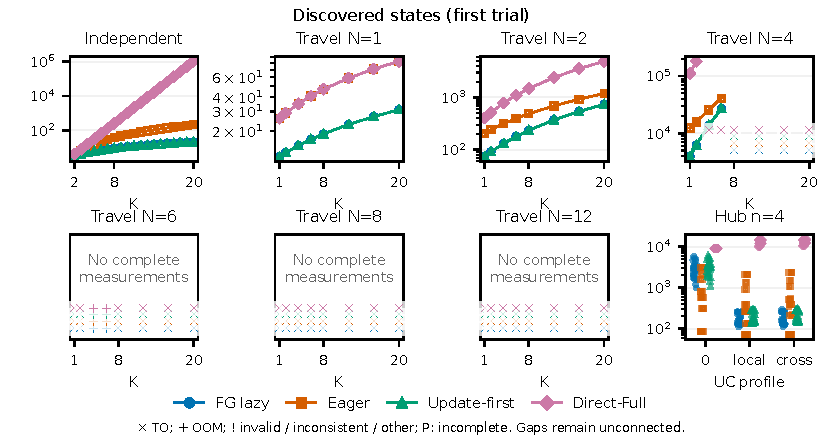
\includegraphics[width=\linewidth]{build/generated/rq4-states-vs-k-full.pdf}
\caption{Full RQ4 state panels, retaining every tested Travel concurrency level and every hub profile. Censored outcomes have status marks and no numeric ordinate.}
\end{figure}
\begin{figure}[p]
\centering
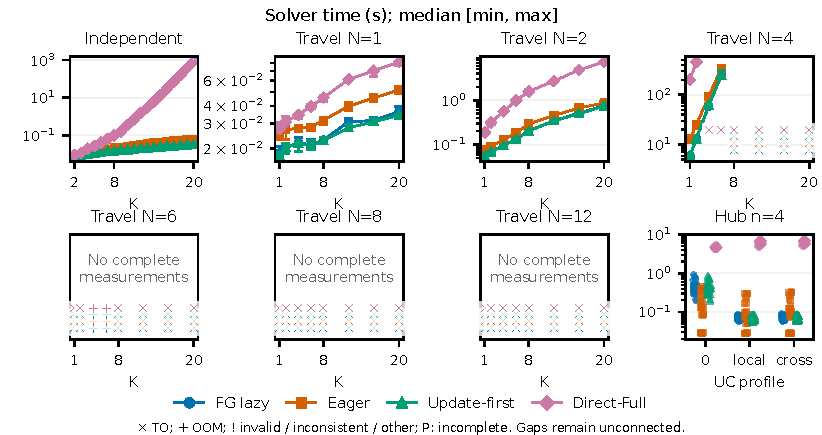
\includegraphics[width=\linewidth]{build/generated/rq4-time-vs-k-full.pdf}
\caption{Full RQ4 time panels. Medians and ranges require five valid, consistent completions; TO/OOM and other incomplete outcomes remain visible.}
\end{figure}
\clearpage

\paragraph{Artifact reproduction status.}
The public anonymous repository contains the full derived source tree, saved RQ1/RQ2 evidence, compiled-monitor exports and Python RS checker, and generated tables/figures. A clean HTTPS clone, build with an empty Maven cache, and RQ1/RQ2 derive-only smoke checks passed; the rederived fields match the saved expectations after path normalization. Tests were compiled but not executed. The README records the environment, elapsed times and anonymized logs in \path{validation/clean-clone/}, separately from the earlier local build evidence. Third-party dependencies are fetched from official upstream sources; no shaded JAR is distributed. Larger raw outputs remain in verified split assets awaiting the \texttt{v2-preview} pre-release, so public asset download/restoration is untested. The final \texttt{fse27-submission} tag will be created after v2 is frozen.

\section{Expanded related-work comparison}
\begin{table}[!htbp]
\caption{Expanded primary-source comparison of verified native contracts. C/R: component/requirement granularity; T: transfer; Res/P: residual obligations/precedence; Roots/O: initial states/outcomes. Publication details are in the main bibliography; section/definition numbers locate the inspected contracts.}
\label{tab:supp-native}
\centering\footnotesize
\setlength{\tabcolsep}{3pt}\renewcommand{\arraystretch}{1.02}
\begin{tabular}{@{}>{\raggedright\arraybackslash}p{.15\linewidth}>{\raggedright\arraybackslash}p{.28\linewidth}>{\raggedright\arraybackslash}p{.29\linewidth}>{\raggedright\arraybackslash}p{.23\linewidth}@{}}
\toprule
Work & Native C/R; T; Res/P & Roots/O; progress premises & Artifact and construction\\
\midrule
DUCS (2016, 2020)
& Global environment/specification switch; set-valued $R$; steps inside $E'$; transition formula $T$ constrains update order (Sec.~4.2)
& All old states via total $H$; all outcomes; eventual update events after hotSwap; legal and deadlock-free (Defs.~4.1--4.3)
& Update controller; FLTL control reduction and MTSA synthesis\\
GR(1) bridge (2022)
& Two specifications and switching assertion; old safety guarantees before switch, new specification afterward
& All prefixes meeting new environment safety; uniformly bounded switch (Def.~3.1); subsequent GR(1) liveness assumes justice
& Symbolic reachability bridge; winning set $W$ or current-state early stop\\
Live Synthesis (2022)
& Old/new LTL and trace or transition system; residual $\Psi(\eta,\varphi)$; old obligations finitely satisfied
& Universal variant: all old finite traces and new traces; reduction assumes one eventual update (Thm.~6.4)
& Obligation monitor and LTL synthesis; LiveLTL language inclusion\\
DES state attraction (2015)
& Common deterministic plant; request/startup sets; task language $K$ and recognizer
& All request states; UC preserved; weakly invariant startup set; bounded first completion (Def.~2, Thm.~1)
& Attractor supervisor; plant/recognizer product and state-attraction algorithm\\
OTF-DCS (2023)
& Component automata, marked/illegal states and control partition
& All UC enabled; designated disturbances; eager director (Def.~3); every finite prefix has a marked extension (Def.~4)
& Safe nonblocking director; heuristic OTF composition\\
Tripakis--Altisen (1999)
& Finite game graph, controllable/UC edges, safe/target sets
& UC-successor closure; controllable path to target from each node (Sec.~2.1); environment may move first
& Strategy subgraph; fully OTF for untimed graphs\\
Strong planning (1998)
& Action/fluent domain, nondeterministic effects and goal formula
& All initial states and outcomes; strong completion; fair iterative extension separate (pp.~40--43)
& OBDD state/action plan; universal outcome preimages; initial-set early stop\\
Dynamic Feature (2024)
& Feature come/go, component reinitialization, simultaneous changes; behavioral/configuration constraints
& Mixed controllability; every reachable state has a path to jointly marked states (Sec.~7)
& CIF BDD synthesis; maximal safe controllable nonblocking supervisor\\
Network updates (2015)
& Per-switch replacement; searched update order; packet-flush waits
& All single-packet traces satisfy LTL; failure freedom, fair forwarding, bounded processing (Sec.~3.1)
& Sequence; DFS and incremental checking; simple/careful completeness\\
\bottomrule
\end{tabular}
\end{table}
\end{document}
